% !TEX program = xelatex
\documentclass[UTF8,fontset=fandol,a4paper,11pt]{ctexart}
\usepackage[margin=21mm,top=23mm,bottom=22mm,headheight=16pt]{geometry}
\usepackage{amsmath,amssymb,mathtools,bm}
\usepackage{tikz}
\usetikzlibrary{arrows.meta,calc,angles,quotes,patterns}
\usepackage{xcolor,booktabs,array,longtable,enumitem,fancyhdr,needspace}
\usepackage[unicode,hidelinks]{hyperref}
\definecolor{ink}{HTML}{24343C}
\definecolor{accent}{HTML}{166A70}
\definecolor{muted}{HTML}{65747A}
\definecolor{rulegray}{HTML}{D4DDE0}
\definecolor{warm}{HTML}{966037}
\color{ink}
\setlength{\parindent}{2em}
\setlength{\parskip}{4pt}
\linespread{1.12}
\AtBeginDocument{\setlength{\abovedisplayskip}{6pt plus 2pt minus 1pt}
\setlength{\belowdisplayskip}{6pt plus 2pt minus 1pt}
\setlength{\abovedisplayshortskip}{0pt plus 1pt}
\setlength{\belowdisplayshortskip}{4pt plus 1pt}}
\setlist[enumerate]{label=(\arabic*),leftmargin=2.3em,itemsep=3pt,topsep=4pt}
\setlist[itemize]{leftmargin=2em,itemsep=2pt,topsep=4pt}
\allowdisplaybreaks[1]
\setlength{\emergencystretch}{2em}
\setcounter{secnumdepth}{0}
\providecommand{\tightlist}{\setlength{\itemsep}{0pt}\setlength{\parskip}{0pt}}
\ctexset{section={format=\Large\bfseries\color{accent},beforeskip=10pt,afterskip=9pt},
subsection={format=\normalsize\bfseries\color{accent},beforeskip=10pt,afterskip=4pt},
subsubsection={format=\normalsize\bfseries,beforeskip=8pt,afterskip=3pt}}
\pagestyle{fancy}
\fancyhf{}
\fancyhead[L]{\small\color{muted}物理学难题集萃}
% 页眉仅保留书名；版本名称只在封面显示。
\fancyfoot[L]{\small\color{muted}\chapterlabel}
\fancyfoot[R]{\small\thepage}
\renewcommand{\headrulewidth}{0.4pt}
\renewcommand{\footrulewidth}{0pt}
\newcommand{\dd}{\mathop{}\!\mathrm{d}}
\newcommand{\vect}[1]{\bm{#1}}
\newcommand{\tagline}[1]{\noindent{\small\color{muted}#1}\par}
\newcommand{\result}[1]{\begin{equation*}\boxed{#1}\end{equation*}}
\newcommand{\figcaption}[1]{\par\vspace{2pt}{\small\color{muted}#1}\par}
\newcommand{\teach}[2]{\Needspace{4\baselineskip}\subsection*{讲解要点与追问}#1\par\smallskip\noindent\textbf{追问：}#2\par}
\newcommand{\workarea}{\par\vspace{7mm}\noindent{\small\color{muted}作答区}\par\vspace{4mm}
\noindent\textcolor{rulegray}{\rule{\linewidth}{0.3pt}}\par\vspace{16mm}
\noindent\textcolor{rulegray}{\rule{\linewidth}{0.3pt}}\par\vspace{16mm}
\noindent\textcolor{rulegray}{\rule{\linewidth}{0.3pt}}\par\vspace{16mm}
\noindent\textcolor{rulegray}{\rule{\linewidth}{0.3pt}}}
\tikzset{axis/.style={-{Stealth[length=2mm]},thin,color=muted},
motion/.style={-{Stealth[length=2.3mm]},thick,color=accent},
force/.style={-{Stealth[length=2.3mm]},thick,color=warm},
traj/.style={thick,color=accent},guide/.style={dashed,thin,color=muted},
object/.style={thick,color=ink},every node/.style={font=\small}}\widowpenalty=10000\clubpenalty=10000\displaywidowpenalty=10000\newcommand{\chapterlabel}{近代物理试题}







\hypersetup{pdftitle={近代物理试题·学生解答版},pdfauthor={}}

\begin{document}\pdfbookmark[0]{近代物理试题}{cover}

\thispagestyle{empty}\vspace*{22mm}

\noindent{\Huge\bfseries 物理学难题集萃}\par\vspace{12mm}

\noindent{\LARGE 近代物理试题}\par\vspace{12mm}

\noindent{\Large\color{accent}学生解答版}\par\vspace{9mm}

\noindent\textcolor{accent}{\rule{\linewidth}{1pt}}\par\vspace{9mm}

\noindent 第1--5题\par\vfill\clearpage

\pdfbookmark[1]{题目目录}{contents}\section*{题目目录}

\begin{longtable}{@{}r p{113mm} r@{}}\toprule 题号 & 题目 & 页码\\\midrule

\hyperref[q:1]{1} & \hyperref[q:1]{热运动和碰撞造成的谱线展宽} & \pageref{q:1} \\

\hyperref[q:2]{2} & \hyperref[q:2]{中子干涉中的重力相位差} & \pageref{q:2} \\

\hyperref[q:3]{3} & \hyperref[q:3]{有限核半径下的缪子原子估算} & \pageref{q:3} \\

\hyperref[q:4]{4} & \hyperref[q:4]{两根运动尺与分别归零的四只钟} & \pageref{q:4} \\

\hyperref[q:5]{5} & \hyperref[q:5]{磁场轨迹与两体反应的粒子鉴别} & \pageref{q:5} \\

\bottomrule\end{longtable}

\clearpage

\pdfbookmark[2]{第 1 题 热运动和碰撞造成的谱线展宽}{q1}

\section*{第 1 题\quad 热运动和碰撞造成的谱线展宽}\label{q:1}


摩尔质量为$\mu$的理想气体处于温度$T$的热平衡态，原子静止时某条谱线中心频率为$\nu_0$、真空波长为$\lambda_0=c/\nu_0$，原子热运动速度远小于$c$。
\begin{enumerate}
\item 从一维麦克斯韦速度分布推导多普勒展宽的归一化频率分布$F(\nu)$。
\item 容器内充氩气，温度$200^\circ\mathrm C$，压强$10\,\mathrm{mmHg}$，含少量钠蒸气。钠灯光通过后出现$\lambda_0=589.6\,\mathrm{nm}$吸收线，钠摩尔质量$23\,\mathrm{g/mol}$。以中心两侧$F(\nu)=F(\nu_0)/\sqrt2$两频率之差定义$\Delta\nu_D$，求对应正的波长宽度。
\item 估计碰撞导致的波长展宽数量级。钠原子有效直径约$0.10\,\mathrm{nm}$；估算时氩原子有效直径取同量级且近似相等，氩摩尔质量取$40\,\mathrm{g/mol}$。说明碰撞率与精确线宽系数的区别。
\end{enumerate}
可用$R=8.314\,\mathrm{J/(mol\,K)}$、$k_B=1.381\times10^{-23}\,\mathrm{J/K}$、
$c=3.00\times10^8\,\mathrm{m/s}$及$1\,\mathrm{mmHg}=133.3\,\mathrm{Pa}$。


\begin{center}\begin{minipage}{.98\linewidth}\centering
\begin{tikzpicture}[scale=.8,transform shape]

\draw[object] (-1,-.6) rectangle (5,1.2);
\node at (2,.85) {氩气与少量钠蒸气};
\draw[motion] (-3,0)--(7,0);
\node[above] at (-2.5,0) {钠灯};\node[above] at (6.5,0) {接收器};
\draw[axis] (-1,-1.2)--(6,-1.2) node[right] {$x$};
\fill (2,0) circle (2pt);\draw[force] (2,.3)--(3.4,.3) node[right] {$v_x$};
\node at (2,2) {$T=200^\circ\mathrm C,\quad p=10\,\mathrm{mmHg}$};

\end{tikzpicture}
\figcaption{图近试.1\quad 接收方向的速度分量造成频移，碰撞限制相干持续时间。}
\end{minipage}\end{center}

\Needspace{6\baselineskip}\subsection*{解答}


图近试.1取由发光或吸收原子指向接收器的方向为$x$，沿该方向的速度分量为$v_x$。一阶多普勒关系为
\[
\nu\simeq\nu_0\left(1+\frac{v_x}{c}\right),
\qquad v_x=c\frac{\nu-\nu_0}{\nu_0}.
\]
对吸收而言，原子所见入射频率满足相同的一阶共振选择关系；速度分布关于零对称，最终线型同样是以$\nu_0$为中心的高斯分布。

相邻波前的到达时间间隔在一阶近似下为$(1-v_x/c)/\nu_0$；取其倒数并展开到$v_x/c$的一次项，得到上面的频移关系。热平衡分子的三个速度分量独立，三维麦氏密度可分解为三个一维高斯因子的乘积。接收方向只选择$v_x$；积分掉横向的$v_y,v_z$后，这两个因子的积分各为1。若单原子质量为$m=\mu/N_A$，由$R=N_Ak_B$，一维密度中的$m/(k_BT)$等于$\mu/(RT)$。因此保留的一维麦克斯韦概率密度为
\[
f(v_x)=\sqrt{\frac{\mu}{2\pi RT}}\,
\exp\left(-\frac{\mu v_x^2}{2RT}\right).
\]
\begin{center}\begin{minipage}{.98\linewidth}\centering
\begin{tikzpicture}[scale=.8,transform shape]

\draw[axis] (-3.5,0)--(4,0) node[right] {$(\nu-\nu_0)/\sigma_\nu$};
\draw[axis] (-3.2,0)--(-3.2,4.8) node[above] {$F/F_0$};
\draw[traj,domain=-3:3,samples=180] plot (\x,{4*exp(-\x*\x/2)});
\draw[guide] (-3.2,2.828427)--(3.2,2.828427);
\draw[guide] (-3.2,2)--(3.2,2);
\node[right] at (3.2,2.828427) {$1/\sqrt2$};
\node[right] at (3.2,2) {$1/2$};
\draw[guide] (-.832555,0)--(-.832555,2.828427);
\draw[guide] (.832555,0)--(.832555,2.828427);
\node[below] at (0,0) {$0$};
\draw[axis,<->] (-.832555,-.8)--(.832555,-.8) node[midway,below] {$\Delta\nu_D/\sigma_\nu$};
\node at (0,5.8) {$F(\nu)d\nu=f(v_x)dv_x,\quad d\nu=\nu_0dv_x/c$};

\end{tikzpicture}
\figcaption{解图近试.1A\quad 题设宽度取0.707倍峰高，区别于通常的半高全宽。}
\end{minipage}\end{center}
解图近试.1A 的横坐标以频率标准差为单位。从速度区间换到频率区间时，同一组原子的概率保持相等，因此
$F(\nu)d\nu=f(v_x)dv_x$。因$dv_x/d\nu=c/\nu_0$，得到
\[
\boxed{F(\nu)=\frac1{\nu_0}
\sqrt{\frac{\mu c^2}{2\pi RT}}
\exp\left[-\frac{\mu c^2}{2RT}
\left(\frac{\nu-\nu_0}{\nu_0}\right)^2\right]}.
\]
雅可比$c/\nu_0$把每单位速度的概率换成每单位频率的概率，使频率分布归一化；$F$的单位为$\mathrm{Hz^{-1}}$。频率标准差为
$\sigma_\nu=(\nu_0/c)\sqrt{RT/\mu}$。令$u=(\nu-\nu_0)/\sigma_\nu$，分布化为$F(\nu)=e^{-u^2/2}/(\sqrt{2\pi}\sigma_\nu)$，用$\int_{-\infty}^{\infty}e^{-u^2/2}\,\mathrm du=\sqrt{2\pi}$即得$\int F(\nu)\,\mathrm d\nu=1$。对称性使平均频率为$\nu_0$，二阶中心矩为$\sigma_\nu^2$；谱线宽度与观察方向的一维热速度标准差对应。

设两个频率端点为$\nu_-<\nu_0<\nu_+$。题设高度$1/\sqrt2$的对数为$-(\ln2)/2$，将峰高比代入高斯指数，求得
\[
\frac{F(\nu_\pm)}{F(\nu_0)}=\frac1{\sqrt2}
\ \Longrightarrow\
\frac{\mu c^2}{2RT}
\left(\frac{\nu_\pm-\nu_0}{\nu_0}\right)^2=\frac{\ln2}{2}.
\]
所以
\[
\nu_\pm-\nu_0=\pm\frac{\nu_0}{c}\sqrt{\frac{RT\ln2}{\mu}},
\qquad
\boxed{\frac{\Delta\nu_D}{\nu_0}
=2\sqrt{\frac{RT\ln2}{\mu c^2}}}.
\]
取$T=473\,\mathrm K$、$\mu=0.023\,\mathrm{kg/mol}$，得
\[
\frac{\Delta\nu_D}{\nu_0}\simeq2.30\times10^{-6}.
\]
由$\lambda=c/\nu$，窄线宽满足$|d\lambda|/\lambda_0=|d\nu|/\nu_0$，频率增大对应波长减小，但宽度取正：
\[
\boxed{\Delta\lambda_D
\simeq\lambda_0\frac{\Delta\nu_D}{\nu_0}
=1.36\times10^{-3}\,\mathrm{nm}}.
\]
也可以直接变换两个端点的波长：令$w=\Delta\nu_D/2$，则短波端为$c/(\nu_0+w)$、长波端为$c/(\nu_0-w)$，两者之差为
\[
\Delta\lambda_D=\frac{2cw}{\nu_0^2-w^2}=\lambda_0\frac{\Delta\nu_D/\nu_0}{1-[\Delta\nu_D/(2\nu_0)]^2}.
\]
本题分母修正量约 $1.3\times10^{-12}$，一阶式和端点转换在所给有效位数内相同。这里转换的是图 A 所选的两个频率端点。若改用按波长计的峰高定义，波长密度要先乘雅可比 $c/\lambda^2$，再从该密度的峰值确定两端。

通常的半高全宽按$F=F_0/2$定义，数值是这里宽度的$\sqrt2$倍。比较不同展宽时，先把它们换成同一峰高定义。
\begin{center}\begin{minipage}{.98\linewidth}\centering
\begin{tikzpicture}[scale=.85,transform shape]

\draw[guide] (0,-.7)--(5,-.7);\draw[guide] (0,.7)--(5,.7);
\draw[guide] (0,0) ellipse (.18 and .7);\draw[guide] (5,0) ellipse (.18 and .7);
\fill[accent!12] (0,-.7) rectangle (5,.7);
\draw[object] (0,0) circle (.35);\node[left] at (-.35,0) {钠};
\draw[motion] (.5,0)--(2,0) node[midway,above] {$\bar u_{\rm rel}$};
\foreach \x/\y in {2.8/.2,4/-.4,3.5/1.6}{\draw[object] (\x,\y) circle (.35);}\node[right] at (4.35,-.4) {氩};
\draw[axis,<->] (0,-1.2)--(5,-1.2) node[midway,below] {$\bar u_{\rm rel}\Delta t$};
\draw[axis,<->] (5.5,0)--(5.5,.7) node[midway,right] {$d_{\rm eff}$};
\node at (2.5,2.5) {$d_{\rm eff}=(d_{\rm Na}+d_{\rm Ar})/2$};
\node at (2.5,-2.7) {$Z=n_{\rm Ar}\pi d_{\rm eff}^2\bar u_{\rm rel}$};

\end{tikzpicture}
\figcaption{解图近试.1B\quad 相对速度扫掠的碰撞管给每个钠原子的平均碰撞率。}
\end{minipage}\end{center}
第（3）问，解图近试.1B用原子间相对运动和有效碰撞截面估计自由飞行时间。氩的数密度与钠、氩约化摩尔质量为
\[
n_{\rm Ar}=\frac p{k_BT}
\simeq2.0\times10^{23}\,\mathrm{m^{-3}},\qquad
\mu_{\rm red}=\frac{\mu_{\rm Na}\mu_{\rm Ar}}
{\mu_{\rm Na}+\mu_{\rm Ar}}
=1.46\times10^{-2}\,\mathrm{kg/mol}.
\]
钠、氩的热运动彼此独立，一维相对速度为$u_x=v_{{\rm Na},x}-v_{{\rm Ar},x}$，其方差等于两方差之和：
\[
\langle u_x^2\rangle=RT\left(\frac1{\mu_{\rm Na}}+\frac1{\mu_{\rm Ar}}\right)=\frac{RT}{\mu_{\rm red}}.
\]
三个相对分量仍是独立高斯，因而相对速率的密度为$4\pi u^2[\mu_{\rm red}/(2\pi RT)]^{3/2}e^{-\mu_{\rm red}u^2/(2RT)}$。乘$u$积分后得到平均相对速率
\[
\bar u_{\rm rel}=\sqrt{\frac{8RT}{\pi\mu_{\rm red}}}
\simeq8.3\times10^2\,\mathrm{m/s}.
\]
一般有效碰撞半径为$(d_{\rm Na}+d_{\rm Ar})/2$，相对运动在单位时间扫过的圆柱体积为$\pi[(d_{\rm Na}+d_{\rm Ar})/2]^2\bar u_{\rm rel}$；乘氩的数密度就是每个钠原子的碰撞数。这里氩占绝大多数，钠—氩碰撞给出主要贡献。两有效直径近似相等为$d=1.0\times10^{-10}\,\mathrm m$，碰撞截面为$\pi d^2$，每个钠原子的平均碰撞率为
\[
Z=\pi d^2n_{\rm Ar}\bar u_{\rm rel}
\simeq5\times10^6\,\mathrm{s^{-1}},\qquad
\tau_{\rm col}\simeq Z^{-1}.
\]
以碰撞间隔限制光波相干持续时间，频宽数量级为
$\Delta\nu_{\rm col}\sim1/\tau_{\rm col}\sim Z$，因而
\[
\boxed{\Delta\lambda_{\rm col}\sim
\frac{\lambda_0^2}{c}Z\sim6\times10^{-6}\,\mathrm{nm}}.
\]
以相干持续时间估得的$1/\tau_{\rm col}$给出频宽数量级；具体峰高对应的宽度系数由相位随机化过程决定。若另指定每次碰撞完全随机化相位、碰撞按泊松过程发生，则场相关函数为$e^{-Z|\tau|}$，其洛伦兹线型的半高全宽是$Z/\pi$；此时波长半高全宽约$2\times10^{-6}\,\mathrm{nm}$。线宽的定义与碰撞对相位的作用决定系数，但都远小于本题的多普勒宽度。
由题给换算，$p=1333\,\mathrm{Pa}$；代入$k_B$和$T$，数密度约$2.04\times10^{23}\,\mathrm{m^{-3}}$。使用未提前取整的约化质量与相对速率，碰撞率约$5.3\times10^6\,\mathrm{s^{-1}}$；上式的$5\times10^6$与$6\times10^{-6}$按有效直径的估算精度取整。

完全随机化的具体线型可从相关函数推导。时间间隔$|t|$内零次碰撞的泊松概率为$e^{-Z|t|}$；发生过碰撞的场相位均匀分布，其相关平均为零，因此$g_1(t)=e^{-Z|t|}$。频谱取它的傅里叶变换，
\[
L(\nu-\nu_0)=2\int_0^\infty e^{-Zt}\cos[2\pi(\nu-\nu_0)t]\,\mathrm dt
=\frac{2Z}{Z^2+[2\pi(\nu-\nu_0)]^2}.
\]
此函数对频率积分为1，峰值为$2/Z$。在半峰高处分母增为两倍，得到$|\nu-\nu_0|=Z/(2\pi)$，两侧全宽为$Z/\pi$；若同样取题设的 $1/\sqrt2$ 高度，频率全宽为 $(Z/\pi)\sqrt{\sqrt2-1}$。用 $Z\simeq5.3\times10^6\,\mathrm{s^{-1}}$ 换算为波长宽度约 $1.3\times10^{-6}\,\mathrm{nm}$，比同一峰高下的多普勒宽度小约三个数量级。解图近试.1C 中，左图的衰减率 $Z$ 决定右图的频率刻度。
\begin{center}\begin{minipage}{.98\linewidth}\centering
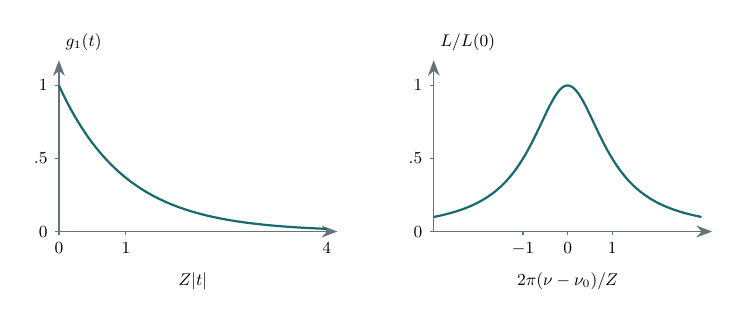
\begin{tikzpicture}[scale=0.68,transform shape]
\draw[axis] (0,0)--(5.2,0);\draw[axis] (0,0)--(0,3.2);
\draw[thin,color=muted] (0.0000000,0)--(0.0000000,-.07);\node[below] at (0.0000000,-.09) {$0$};
\draw[thin,color=muted] (1.2500000,0)--(1.2500000,-.07);\node[below] at (1.2500000,-.09) {$1$};
\draw[thin,color=muted] (5.0000000,0)--(5.0000000,-.07);\node[below] at (5.0000000,-.09) {$4$};
\draw[thin,color=muted] (0,0.0000000)--(-.07,0.0000000);\node[left] at (-.09,0.0000000) {$0$};
\draw[thin,color=muted] (0,1.3636364)--(-.07,1.3636364);\node[left] at (-.09,1.3636364) {$.5$};
\draw[thin,color=muted] (0,2.7272727)--(-.07,2.7272727);\node[left] at (-.09,2.7272727) {$1$};
\node[below] at (2.5,-.64) {$Z|t|$};\node[above right] at (0,3.25) {$g_1(t)$};
\draw[traj] plot coordinates {(0.0000000,2.7272727) (0.0250000,2.6732691) (0.0500000,2.6203348) (0.0750000,2.5684487) (0.1000000,2.5175900) (0.1250000,2.4677384) (0.1500000,2.4188739) (0.1750000,2.3709770) (0.2000000,2.3240285) (0.2250000,2.2780097) (0.2500000,2.2329021) (0.2750000,2.1886876) (0.3000000,2.1453487) (0.3250000,2.1028680) (0.3500000,2.0612284) (0.3750000,2.0204133) (0.4000000,1.9804065) (0.4250000,1.9411918) (0.4500000,1.9027536) (0.4750000,1.8650766) (0.5000000,1.8281456) (0.5250000,1.7919459) (0.5500000,1.7564630) (0.5750000,1.7216827) (0.6000000,1.6875911) (0.6250000,1.6541745) (0.6500000,1.6214197) (0.6750000,1.5893134) (0.7000000,1.5578429) (0.7250000,1.5269955) (0.7500000,1.4967590) (0.7750000,1.4671212) (0.8000000,1.4380702) (0.8250000,1.4095945) (0.8500000,1.3816827) (0.8750000,1.3543236) (0.9000000,1.3275062) (0.9250000,1.3012198) (0.9500000,1.2754539) (0.9750000,1.2501982) (1.0000000,1.2254426) (1.0250000,1.2011772) (1.0500000,1.1773923) (1.0750000,1.1540784) (1.1000000,1.1312261) (1.1250000,1.1088263) (1.1500000,1.0868701) (1.1750000,1.0653486) (1.2000000,1.0442533) (1.2250000,1.0235757) (1.2500000,1.0033076) (1.2750000,0.9834407) (1.3000000,0.9639673) (1.3250000,0.9448795) (1.3500000,0.9261696) (1.3750000,0.9078302) (1.4000000,0.8898540) (1.4250000,0.8722337) (1.4500000,0.8549623) (1.4750000,0.8380329) (1.5000000,0.8214388) (1.5250000,0.8051732) (1.5500000,0.7892297) (1.5750000,0.7736019) (1.6000000,0.7582835) (1.6250000,0.7432685) (1.6500000,0.7285508) (1.6750000,0.7141246) (1.7000000,0.6999839) (1.7250000,0.6861233) (1.7500000,0.6725372) (1.7750000,0.6592200) (1.8000000,0.6461666) (1.8250000,0.6333717) (1.8500000,0.6208301) (1.8750000,0.6085368) (1.9000000,0.5964870) (1.9250000,0.5846757) (1.9500000,0.5730984) (1.9750000,0.5617503) (2.0000000,0.5506269) (2.0250000,0.5397237) (2.0500000,0.5290365) (2.0750000,0.5185609) (2.1000000,0.5082927) (2.1250000,0.4982278) (2.1500000,0.4883622) (2.1750000,0.4786920) (2.2000000,0.4692133) (2.2250000,0.4599222) (2.2500000,0.4508151) (2.2750000,0.4418884) (2.3000000,0.4331384) (2.3250000,0.4245617) (2.3500000,0.4161548) (2.3750000,0.4079144) (2.4000000,0.3998372) (2.4250000,0.3919199) (2.4500000,0.3841593) (2.4750000,0.3765525) (2.5000000,0.3690962) (2.5250000,0.3617876) (2.5500000,0.3546238) (2.5750000,0.3476017) (2.6000000,0.3407188) (2.6250000,0.3339721) (2.6500000,0.3273590) (2.6750000,0.3208768) (2.7000000,0.3145231) (2.7250000,0.3082951) (2.7500000,0.3021904) (2.7750000,0.2962067) (2.8000000,0.2903414) (2.8250000,0.2845922) (2.8500000,0.2789569) (2.8750000,0.2734332) (2.9000000,0.2680189) (2.9250000,0.2627117) (2.9500000,0.2575097) (2.9750000,0.2524107) (3.0000000,0.2474126) (3.0250000,0.2425135) (3.0500000,0.2377114) (3.0750000,0.2330044) (3.1000000,0.2283906) (3.1250000,0.2238682) (3.1500000,0.2194353) (3.1750000,0.2150902) (3.2000000,0.2108311) (3.2250000,0.2066564) (3.2500000,0.2025643) (3.2750000,0.1985533) (3.3000000,0.1946216) (3.3250000,0.1907679) (3.3500000,0.1869904) (3.3750000,0.1832878) (3.4000000,0.1796584) (3.4250000,0.1761009) (3.4500000,0.1726139) (3.4750000,0.1691959) (3.5000000,0.1658456) (3.5250000,0.1625617) (3.5500000,0.1593427) (3.5750000,0.1561875) (3.6000000,0.1530948) (3.6250000,0.1500633) (3.6500000,0.1470919) (3.6750000,0.1441793) (3.7000000,0.1413243) (3.7250000,0.1385259) (3.7500000,0.1357829) (3.7750000,0.1330942) (3.8000000,0.1304588) (3.8250000,0.1278755) (3.8500000,0.1253434) (3.8750000,0.1228615) (3.9000000,0.1204286) (3.9250000,0.1180440) (3.9500000,0.1157066) (3.9750000,0.1134154) (4.0000000,0.1111696) (4.0250000,0.1089683) (4.0500000,0.1068106) (4.0750000,0.1046956) (4.1000000,0.1026225) (4.1250000,0.1005905) (4.1500000,0.0985986) (4.1750000,0.0966462) (4.2000000,0.0947325) (4.2250000,0.0928567) (4.2500000,0.0910180) (4.2750000,0.0892157) (4.3000000,0.0874491) (4.3250000,0.0857175) (4.3500000,0.0840202) (4.3750000,0.0823565) (4.4000000,0.0807257) (4.4250000,0.0791273) (4.4500000,0.0775604) (4.4750000,0.0760246) (4.5000000,0.0745192) (4.5250000,0.0730437) (4.5500000,0.0715973) (4.5750000,0.0701796) (4.6000000,0.0687899) (4.6250000,0.0674278) (4.6500000,0.0660926) (4.6750000,0.0647839) (4.7000000,0.0635011) (4.7250000,0.0622437) (4.7500000,0.0610112) (4.7750000,0.0598031) (4.8000000,0.0586189) (4.8250000,0.0574582) (4.8500000,0.0563204) (4.8750000,0.0552052) (4.9000000,0.0541121) (4.9250000,0.0530406) (4.9500000,0.0519903) (4.9750000,0.0509608) (5.0000000,0.0499517)};
\begin{scope}[xshift=7cm]\draw[axis] (0,0)--(5.2,0);\draw[axis] (0,0)--(0,3.2);
\draw[thin,color=muted] (1.6666667,0)--(1.6666667,-.07);\node[below] at (1.6666667,-.09) {$-1$};
\draw[thin,color=muted] (2.5000000,0)--(2.5000000,-.07);\node[below] at (2.5000000,-.09) {$0$};
\draw[thin,color=muted] (3.3333333,0)--(3.3333333,-.07);\node[below] at (3.3333333,-.09) {$1$};
\draw[thin,color=muted] (0,0.0000000)--(-.07,0.0000000);\node[left] at (-.09,0.0000000) {$0$};
\draw[thin,color=muted] (0,1.3636364)--(-.07,1.3636364);\node[left] at (-.09,1.3636364) {$.5$};
\draw[thin,color=muted] (0,2.7272727)--(-.07,2.7272727);\node[left] at (-.09,2.7272727) {$1$};
\node[below] at (2.5,-.64) {$2\pi(\nu-\nu_0)/Z$};\node[above right] at (0,3.25) {$L/L(0)$};
\draw[traj] plot coordinates {(0.0000000,0.2727273) (0.0166667,0.2760286) (0.0333333,0.2793879) (0.0500000,0.2828065) (0.0666667,0.2862858) (0.0833333,0.2898271) (0.1000000,0.2934318) (0.1166667,0.2971015) (0.1333333,0.3008375) (0.1500000,0.3046415) (0.1666667,0.3085150) (0.1833333,0.3124596) (0.2000000,0.3164771) (0.2166667,0.3205690) (0.2333333,0.3247372) (0.2500000,0.3289834) (0.2666667,0.3333096) (0.2833333,0.3377177) (0.3000000,0.3422095) (0.3166667,0.3467871) (0.3333333,0.3514527) (0.3500000,0.3562082) (0.3666667,0.3610560) (0.3833333,0.3659983) (0.4000000,0.3710373) (0.4166667,0.3761755) (0.4333333,0.3814154) (0.4500000,0.3867594) (0.4666667,0.3922102) (0.4833333,0.3977704) (0.5000000,0.4034427) (0.5166667,0.4092300) (0.5333333,0.4151353) (0.5500000,0.4211614) (0.5666667,0.4273115) (0.5833333,0.4335887) (0.6000000,0.4399962) (0.6166667,0.4465375) (0.6333333,0.4532160) (0.6500000,0.4600352) (0.6666667,0.4669988) (0.6833333,0.4741104) (0.7000000,0.4813740) (0.7166667,0.4887936) (0.7333333,0.4963732) (0.7500000,0.5041170) (0.7666667,0.5120293) (0.7833333,0.5201146) (0.8000000,0.5283774) (0.8166667,0.5368224) (0.8333333,0.5454545) (0.8500000,0.5542787) (0.8666667,0.5632999) (0.8833333,0.5725235) (0.9000000,0.5819547) (0.9166667,0.5915993) (0.9333333,0.6014628) (0.9500000,0.6115510) (0.9666667,0.6218699) (0.9833333,0.6324257) (1.0000000,0.6432247) (1.0166667,0.6542733) (1.0333333,0.6655781) (1.0500000,0.6771459) (1.0666667,0.6889836) (1.0833333,0.7010984) (1.1000000,0.7134975) (1.1166667,0.7261883) (1.1333333,0.7391784) (1.1500000,0.7524756) (1.1666667,0.7660878) (1.1833333,0.7800231) (1.2000000,0.7942896) (1.2166667,0.8088957) (1.2333333,0.8238499) (1.2500000,0.8391608) (1.2666667,0.8548372) (1.2833333,0.8708880) (1.3000000,0.8873219) (1.3166667,0.9041482) (1.3333333,0.9213759) (1.3500000,0.9390142) (1.3666667,0.9570721) (1.3833333,0.9755590) (1.4000000,0.9944839) (1.4166667,1.0138560) (1.4333333,1.0336843) (1.4500000,1.0539777) (1.4666667,1.0747449) (1.4833333,1.0959945) (1.5000000,1.1177347) (1.5166667,1.1399736) (1.5333333,1.1627186) (1.5500000,1.1859770) (1.5666667,1.2097555) (1.5833333,1.2340601) (1.6000000,1.2588962) (1.6166667,1.2842686) (1.6333333,1.3101810) (1.6500000,1.3366363) (1.6666667,1.3636364) (1.6833333,1.3911818) (1.7000000,1.4192718) (1.7166667,1.4479044) (1.7333333,1.4770758) (1.7500000,1.5067805) (1.7666667,1.5370112) (1.7833333,1.5677585) (1.8000000,1.5990107) (1.8166667,1.6307538) (1.8333333,1.6629712) (1.8500000,1.6956433) (1.8666667,1.7287479) (1.8833333,1.7622595) (1.9000000,1.7961491) (1.9166667,1.8303844) (1.9333333,1.8649294) (1.9500000,1.8997442) (1.9666667,1.9347849) (1.9833333,1.9700034) (2.0000000,2.0053476) (2.0166667,2.0407608) (2.0333333,2.0761820) (2.0500000,2.1115459) (2.0666667,2.1467827) (2.0833333,2.1818182) (2.1000000,2.2165741) (2.1166667,2.2509679) (2.1333333,2.2849135) (2.1500000,2.3183209) (2.1666667,2.3510972) (2.1833333,2.3831464) (2.2000000,2.4143703) (2.2166667,2.4446690) (2.2333333,2.4739412) (2.2500000,2.5020851) (2.2666667,2.5289992) (2.2833333,2.5545829) (2.3000000,2.5787375) (2.3166667,2.6013666) (2.3333333,2.6223776) (2.3500000,2.6416822) (2.3666667,2.6591973) (2.3833333,2.6748458) (2.4000000,2.6885575) (2.4166667,2.7002700) (2.4333333,2.7099292) (2.4500000,2.7174898) (2.4666667,2.7229161) (2.4833333,2.7261823) (2.5000000,2.7272727) (2.5166667,2.7261823) (2.5333333,2.7229161) (2.5500000,2.7174898) (2.5666667,2.7099292) (2.5833333,2.7002700) (2.6000000,2.6885575) (2.6166667,2.6748458) (2.6333333,2.6591973) (2.6500000,2.6416822) (2.6666667,2.6223776) (2.6833333,2.6013666) (2.7000000,2.5787375) (2.7166667,2.5545829) (2.7333333,2.5289992) (2.7500000,2.5020851) (2.7666667,2.4739412) (2.7833333,2.4446690) (2.8000000,2.4143703) (2.8166667,2.3831464) (2.8333333,2.3510972) (2.8500000,2.3183209) (2.8666667,2.2849135) (2.8833333,2.2509679) (2.9000000,2.2165741) (2.9166667,2.1818182) (2.9333333,2.1467827) (2.9500000,2.1115459) (2.9666667,2.0761820) (2.9833333,2.0407608) (3.0000000,2.0053476) (3.0166667,1.9700034) (3.0333333,1.9347849) (3.0500000,1.8997442) (3.0666667,1.8649294) (3.0833333,1.8303844) (3.1000000,1.7961491) (3.1166667,1.7622595) (3.1333333,1.7287479) (3.1500000,1.6956433) (3.1666667,1.6629712) (3.1833333,1.6307538) (3.2000000,1.5990107) (3.2166667,1.5677585) (3.2333333,1.5370112) (3.2500000,1.5067805) (3.2666667,1.4770758) (3.2833333,1.4479044) (3.3000000,1.4192718) (3.3166667,1.3911818) (3.3333333,1.3636364) (3.3500000,1.3366363) (3.3666667,1.3101810) (3.3833333,1.2842686) (3.4000000,1.2588962) (3.4166667,1.2340601) (3.4333333,1.2097555) (3.4500000,1.1859770) (3.4666667,1.1627186) (3.4833333,1.1399736) (3.5000000,1.1177347) (3.5166667,1.0959945) (3.5333333,1.0747449) (3.5500000,1.0539777) (3.5666667,1.0336843) (3.5833333,1.0138560) (3.6000000,0.9944839) (3.6166667,0.9755590) (3.6333333,0.9570721) (3.6500000,0.9390142) (3.6666667,0.9213759) (3.6833333,0.9041482) (3.7000000,0.8873219) (3.7166667,0.8708880) (3.7333333,0.8548372) (3.7500000,0.8391608) (3.7666667,0.8238499) (3.7833333,0.8088957) (3.8000000,0.7942896) (3.8166667,0.7800231) (3.8333333,0.7660878) (3.8500000,0.7524756) (3.8666667,0.7391784) (3.8833333,0.7261883) (3.9000000,0.7134975) (3.9166667,0.7010984) (3.9333333,0.6889836) (3.9500000,0.6771459) (3.9666667,0.6655781) (3.9833333,0.6542733) (4.0000000,0.6432247) (4.0166667,0.6324257) (4.0333333,0.6218699) (4.0500000,0.6115510) (4.0666667,0.6014628) (4.0833333,0.5915993) (4.1000000,0.5819547) (4.1166667,0.5725235) (4.1333333,0.5632999) (4.1500000,0.5542787) (4.1666667,0.5454545) (4.1833333,0.5368224) (4.2000000,0.5283774) (4.2166667,0.5201146) (4.2333333,0.5120293) (4.2500000,0.5041170) (4.2666667,0.4963732) (4.2833333,0.4887936) (4.3000000,0.4813740) (4.3166667,0.4741104) (4.3333333,0.4669988) (4.3500000,0.4600352) (4.3666667,0.4532160) (4.3833333,0.4465375) (4.4000000,0.4399962) (4.4166667,0.4335887) (4.4333333,0.4273115) (4.4500000,0.4211614) (4.4666667,0.4151353) (4.4833333,0.4092300) (4.5000000,0.4034427) (4.5166667,0.3977704) (4.5333333,0.3922102) (4.5500000,0.3867594) (4.5666667,0.3814154) (4.5833333,0.3761755) (4.6000000,0.3710373) (4.6166667,0.3659983) (4.6333333,0.3610560) (4.6500000,0.3562082) (4.6666667,0.3514527) (4.6833333,0.3467871) (4.7000000,0.3422095) (4.7166667,0.3377177) (4.7333333,0.3333096) (4.7500000,0.3289834) (4.7666667,0.3247372) (4.7833333,0.3205690) (4.8000000,0.3164771) (4.8166667,0.3124596) (4.8333333,0.3085150) (4.8500000,0.3046415) (4.8666667,0.3008375) (4.8833333,0.2971015) (4.9000000,0.2934318) (4.9166667,0.2898271) (4.9333333,0.2862858) (4.9500000,0.2828065) (4.9666667,0.2793879) (4.9833333,0.2760286) (5.0000000,0.2727273)};
\end{scope}\end{tikzpicture}
\figcaption{解图近试.1C\quad 完全随机化碰撞的指数场相关函数与归一峰高的洛伦兹谱}
\end{minipage}\end{center}


\Needspace{13\baselineskip}

\pdfbookmark[2]{第 2 题 中子干涉中的重力相位差}{q2}

\section*{第 2 题\quad 中子干涉中的重力相位差}\label{q:2}


四个光路结点$B,C,E,D$构成菱形，$BC=CE=ED=DB=l$，对角线$BE$分别与$BC$、$BD$夹角$\theta$。平行单晶片在$B$分束，使两束低能中子分别沿$BCE$与$BDE$传播，在$E$合束后由探测器$F$计数。

装置平面$S$可绕$BD$轴旋转，相对水平面$S_0$的有向夹角为$\phi\in[-90^\circ,90^\circ]$；规定$\phi>0$时$C,E$高于$B,D$。重力势能变化远小于中子初动能，忽略光路的微小重力弯曲。
\begin{enumerate}
\item 证明重力相位差可写成$\delta=q\sin\phi$、$q=k\lambda l^2\sin2\theta$，求常数$k$；相位差定义为下路径减上路径，$\lambda$为入射波长。
\item 初动能为$3.9\times10^{-2}\,\mathrm{eV}$，$l=4.0\,\mathrm{cm}$、$\theta=22.5^\circ$，估计旋转全程相长极大的次数。分别说明固定附加相位未知，以及已校准$\phi=0$为相长极大时的答案。
\end{enumerate}
可用中子静能$mc^2=939\,\mathrm{MeV}$、$\hbar c=1.97\times10^{-11}\,\mathrm{MeV\,cm}$、$g=9.8\,\mathrm{m/s^2}$。


\begin{center}\begin{minipage}{.98\linewidth}\centering
\begin{tikzpicture}[scale=.65,transform shape]

\coordinate (B) at (0,0);\coordinate (D) at (4,0);
\coordinate (C) at (2.828,2.828);\coordinate (E) at (6.828,2.828);
\draw[object] (B)--(C)--(E)--(D)--cycle;
\draw[guide,line width=1.2pt] (B)--(E);
\draw[guide,line width=1.2pt] (2.2,2.568)--(3.456,3.088);
\draw[guide,line width=1.2pt] (3.372,-.26)--(4.628,.26);
\draw[motion] (-1.5,0)--(B) node[midway,above] {$A$};
\draw[motion] (C)--(4.8,2.828);
\draw[motion] (D)--(5.6,1.6);
\draw[motion] (E)--(8,2.828) node[right] {$F$};
\foreach \p/\pos in {B/below left,C/above left,E/above,D/below right}{\fill (\p) circle (1.5pt) node[\pos] {$\p$};}
\node[below] at (2,0) {$l$};\node[above] at (4.8,2.828) {$l$};
\node[left] at (1.4,1.5) {$l$};\node[right] at (5.6,1.5) {$l$};
\draw[object] (1.2,0) arc[start angle=0,end angle=22.5,radius=1.2];
\draw[object] (22.5:1.6) arc[start angle=22.5,end angle=45,radius=1.6];
\node at (1.4,.2) {$\theta$};\node at (1.65,1.05) {$\theta$};
\begin{scope}[xshift=10cm]
\draw[guide] (-1,0)--(3,0) node[right] {$S_0$};
\draw[object] (0,0)--(2.5,1.5) node[right] {$S$};
\fill (0,0) circle (2pt) node[below] {$BD$轴};
\node at (1,.3) {$\phi$};
\end{scope}

\end{tikzpicture}
\figcaption{图近试.2\quad 菱形光路的平面内几何与绕BD旋转的侧视示意。}
\end{minipage}\end{center}

\Needspace{6\baselineskip}\subsection*{解答}


图近试.2中菱形面积为$A=l^2\sin2\theta$。绕$BD$旋转后，$CE$比$BD$高
\[
h=l\sin2\theta\sin\phi.
\]
在装置平面内，$BE$平分菱形顶角，所以$BC$与$BD$的夹角为$2\theta$，$C$到转轴$BD$的垂距为$l\sin2\theta$。旋转只把这个平面内垂距的竖直分量乘$\sin\phi$，因而上面的高度和面积都由实际菱形几何确定。弹性分束和反射不改变中子的总机械能。下侧水平段$BD$的动量为$p_0=mv_0=h_{\rm P}/\lambda$，这里$h_{\rm P}=2\pi\hbar$为普朗克常量；上侧段$CE$动量为
\[
p_2=\sqrt{p_0^2-2m^2gh}
=p_0\sqrt{1-\frac{2m^2gh}{p_0^2}}.
\]
在$|mgh|\ll p_0^2/(2m)$下，
\[
p_0-p_2\simeq\frac{m^2gh}{p_0}
=\frac{mgh}{v_0}.
\]
\begin{center}\begin{minipage}{.98\linewidth}\centering
\begin{tikzpicture}[scale=.8,transform shape]

\draw[object] (0,0)--(4,0);\draw[object] (0,3)--(4,3);
\draw[motion] (.7,0)--(2,0) node[midway,below] {$p_0$};
\draw[motion] (2,3)--(3.3,3) node[midway,above] {$p_2$};
\draw[guide] (0,0)--(0,3);\draw[guide] (4,0)--(4,3);
\node[below left] at (0,0) {$B$};\node[below right] at (4,0) {$D$};
\node[above left] at (0,3) {$C$};\node[above right] at (4,3) {$E$};
\draw[axis,<->] (-1,0)--(-1,3) node[midway,left] {$h$};
\draw[axis,<->] (0,-1)--(4,-1) node[midway,below] {$l$};
\node[align=left] at (7,2) {$h=l\sin2\theta\sin\phi$\\$BC,DE$高度历程相同\\高、低两等长边有动量差};
\node at (2,4.5) {将两斜边配对后，仅比较两个水平段的相位};

\end{tikzpicture}
\figcaption{解图近试.2A\quad 相位积分的配对展开图；虚线对应高度历程相同的两条实际斜边。}
\end{minipage}\end{center}
解图近试.2A把两条斜边与两条等高边分别配对。$BC$与$DE$都从低处走向高处，长度、沿路高度变化一致，因此定能量相位积分$\int p\,ds/\hbar$的这两段相消。具体地，用各斜边从低端起的弧长$s$作参数，两条斜边的高度都是$hs/l$，它们的相位都为$\hbar^{-1}\int_0^l\sqrt{p_0^2-2m^2ghs/l}\,\mathrm ds$。两条相同积分在下减上的相位差中抵消，只剩$BD$与$CE$各长$l$的差：
\[
\begin{aligned}
\delta&=\frac l\hbar(p_0-p_2)
\simeq\frac{mglh}{\hbar v_0}\\
&=\frac{mg\,l^2\sin2\theta}{\hbar v_0}\sin\phi.
\end{aligned}
\]
从速度形式也能看出同一动量差：能量守恒给出$(v_0-v_2)(v_0+v_2)=2gh$，小势能变化下取$v_0+v_2\simeq2v_0$，得$v_0-v_2\simeq gh/v_0$。代入$2\pi l(1/\lambda-1/\lambda_2)=ml(v_0-v_2)/\hbar$，正好得到上式。

用$v_0=h_{\rm P}/(m\lambda)=2\pi\hbar/(m\lambda)$代入，
\[
\boxed{\delta=q\sin\phi,\qquad
q=\frac{m^2g}{2\pi\hbar^2}\lambda l^2\sin2\theta},
\qquad
\boxed{k=\frac{m^2g}{2\pi\hbar^2}}.
\]
在SI中$k$的量纲为$\mathrm{m^{-3}}$，与$\lambda l^2$相乘后相位无量纲。$k$只涉及中子质量、重力加速度和$\hbar$；几何面积和波长已单独列出。若改定义相位为上路径减下路径，整体变号，干涉强度的物理结论不变。

第（2）问，由非相对论动能
\[
E_k=\frac{p_0^2}{2m},\qquad
\lambda=\frac{2\pi\hbar c}{\sqrt{2mc^2E_k}}.
\]
将$E_k=3.9\times10^{-8}\,\mathrm{MeV}$代入，
\[
\lambda=
\frac{2\pi(1.97\times10^{-11})}
{\sqrt{2\times939\times3.9\times10^{-8}}}\,\mathrm{cm}
\simeq1.45\times10^{-8}\,\mathrm{cm}
=0.145\,\mathrm{nm}.
\]
再用一致的长度、能量单位代入相位系数，得
\[
\boxed{\frac q{2\pi}\simeq10.3}.
\]
由$\phi=-90^\circ$至$90^\circ$，$\sin\phi$单调从$-1$到$1$，相位$\delta/(2\pi)$覆盖约$[-10.3,10.3]$，总跨度约$20.6$个周期。
\begin{center}\begin{minipage}{.98\linewidth}\centering
\begin{tikzpicture}[scale=.85,transform shape]

\foreach \y in {1.4,-1.4}{
\draw[axis] (-5,\y)--(5,\y);
\draw[object] (-4.12,{\y-.2})--(-4.12,{\y+.2});
\draw[object] (4.12,{\y-.2})--(4.12,{\y+.2});}
\foreach \n in {-10,...,10}{\fill ({.4*\n},1.4) circle (1.8pt);}
\foreach \n in {-10,...,9}{\fill ({.4*(\n+.5)},-1.4) circle (1.8pt);}
\node at (0,2.6) {$\delta_0=0$：21个相长整数点};
\node at (0,-.2) {$\delta_0=\pi$：20个相长点};
\node[below] at (-4.12,-1.6) {$-q/(2\pi)$};
\node[below] at (4.12,-1.6) {$q/(2\pi)$};
\node at (0,-3) {可达相位区间长度约20.6；两种图示情形的端点均位于峰间};

\end{tikzpicture}
\figcaption{解图近试.2B\quad 固定相位平移相长格点；零角校准后可唯一数出21个。}
\end{minipage}\end{center}
解图近试.2B将可达到的相位区间与相长整数点相比。计数率还包含固定的装置相位，可写为
\[
I_F=I_{\rm av}[1+\mathcal V\cos(\delta+\delta_0)],
\]
其中$\delta_0$是固定的晶体反射、分束等附加相位。极大条件为
$\delta+\delta_0=2\pi n$。当$\delta_0$未给定时，一个长度约$20.6$的区间可容纳20或21个整数，故相长极大次数为
\[
\boxed{20\ \text{次或}\ 21\ \text{次，取决于固定相位}}.
\]
若已校准$\phi=0$为相长极大，则$\delta_0\equiv0\pmod{2\pi}$，整数为$n=-10,-9,\ldots,10$，共
\[
\boxed{21\ \text{次}}.
\]
约20.6个周期给出相位区间长度；经过的相长中心数由该区间内的整数格点逐个计出。
将固定相位记为$a=\delta_0/(2\pi)$，相长条件对应整数$n$满足$a-Q\leqslant n\leqslant a+Q$，$Q=q/(2\pi)$；包含端点时的数目为$\lfloor a+Q\rfloor-\lceil a-Q\rceil+1$。将 $a$ 取在 $[-1/2,1/2]$，图 B 中的相长格点随 $a$ 移动。只要 $|a|\le Q-10\simeq0.3$，两个整数 $-10$ 和 $10$ 都在可达区间里，从 $-10$ 到 $10$ 共 $21$ 次；再向任一侧平移，恰有一个端点整数移出，剩 $20$ 次。校准零角时 $a=0$，转角单调变化，每个相长格点只经过一次。解图近试.2C把对应相长角$\phi_n=\arcsin(n/Q)$标在相位曲线上，显示转角间距在两端增大。
\begin{center}\begin{minipage}{.98\linewidth}\centering
\begin{tikzpicture}[scale=0.72,transform shape]
\draw[axis] (0,0)--(6.2,0);\draw[axis] (0,0)--(0,3.4000000000000004);
\draw[thin,color=muted] (0.0000000,0)--(0.0000000,-.07);\node[below] at (0.0000000,-.09) {$-90$};
\draw[thin,color=muted] (3.0000000,0)--(3.0000000,-.07);\node[below] at (3.0000000,-.09) {$0$};
\draw[thin,color=muted] (6.0000000,0)--(6.0000000,-.07);\node[below] at (6.0000000,-.09) {$90$};
\draw[thin,color=muted] (0,0.1454545)--(-.07,0.1454545);\node[left] at (-.09,0.1454545) {$-10$};
\draw[thin,color=muted] (0,1.6000000)--(-.07,1.6000000);\node[left] at (-.09,1.6000000) {$0$};
\draw[thin,color=muted] (0,3.0545455)--(-.07,3.0545455);\node[left] at (-.09,3.0545455) {$10$};
\node[below] at (3.0,-.64) {转角$\phi$（度）};\node[above right] at (0,3.45) {$\delta/(2\pi)$};
\draw[traj] plot coordinates {(0.0000000,0.1018182) (0.0166667,0.1018752) (0.0333333,0.1020464) (0.0500000,0.1023316) (0.0666667,0.1027308) (0.0833333,0.1032441) (0.1000000,0.1038714) (0.1166667,0.1046126) (0.1333333,0.1054677) (0.1500000,0.1064366) (0.1666667,0.1075192) (0.1833333,0.1087155) (0.2000000,0.1100254) (0.2166667,0.1114487) (0.2333333,0.1129854) (0.2500000,0.1146353) (0.2666667,0.1163984) (0.2833333,0.1182744) (0.3000000,0.1202633) (0.3166667,0.1223648) (0.3333333,0.1245789) (0.3500000,0.1269054) (0.3666667,0.1293440) (0.3833333,0.1318946) (0.4000000,0.1345570) (0.4166667,0.1373311) (0.4333333,0.1402165) (0.4500000,0.1432131) (0.4666667,0.1463206) (0.4833333,0.1495388) (0.5000000,0.1528675) (0.5166667,0.1563064) (0.5333333,0.1598552) (0.5500000,0.1635137) (0.5666667,0.1672816) (0.5833333,0.1711586) (0.6000000,0.1751444) (0.6166667,0.1792387) (0.6333333,0.1834413) (0.6500000,0.1877517) (0.6666667,0.1921696) (0.6833333,0.1966948) (0.7000000,0.2013268) (0.7166667,0.2060653) (0.7333333,0.2109100) (0.7500000,0.2158605) (0.7666667,0.2209164) (0.7833333,0.2260773) (0.8000000,0.2313428) (0.8166667,0.2367126) (0.8333333,0.2421862) (0.8500000,0.2477631) (0.8666667,0.2534431) (0.8833333,0.2592256) (0.9000000,0.2651102) (0.9166667,0.2710965) (0.9333333,0.2771840) (0.9500000,0.2833722) (0.9666667,0.2896607) (0.9833333,0.2960489) (1.0000000,0.3025365) (1.0166667,0.3091229) (1.0333333,0.3158075) (1.0500000,0.3225900) (1.0666667,0.3294698) (1.0833333,0.3364463) (1.1000000,0.3435190) (1.1166667,0.3506874) (1.1333333,0.3579510) (1.1500000,0.3653091) (1.1666667,0.3727613) (1.1833333,0.3803069) (1.2000000,0.3879454) (1.2166667,0.3956763) (1.2333333,0.4034988) (1.2500000,0.4114125) (1.2666667,0.4194166) (1.2833333,0.4275107) (1.3000000,0.4356941) (1.3166667,0.4439661) (1.3333333,0.4523261) (1.3500000,0.4607736) (1.3666667,0.4693078) (1.3833333,0.4779282) (1.4000000,0.4866339) (1.4166667,0.4954245) (1.4333333,0.5042992) (1.4500000,0.5132573) (1.4666667,0.5222982) (1.4833333,0.5314211) (1.5000000,0.5406255) (1.5166667,0.5499105) (1.5333333,0.5592755) (1.5500000,0.5687197) (1.5666667,0.5782425) (1.5833333,0.5878430) (1.6000000,0.5975207) (1.6166667,0.6072747) (1.6333333,0.6171043) (1.6500000,0.6270087) (1.6666667,0.6369873) (1.6833333,0.6470392) (1.7000000,0.6571636) (1.7166667,0.6673599) (1.7333333,0.6776272) (1.7500000,0.6879647) (1.7666667,0.6983717) (1.7833333,0.7088473) (1.8000000,0.7193908) (1.8166667,0.7300014) (1.8333333,0.7406782) (1.8500000,0.7514205) (1.8666667,0.7622274) (1.8833333,0.7730980) (1.9000000,0.7840317) (1.9166667,0.7950275) (1.9333333,0.8060846) (1.9500000,0.8172022) (1.9666667,0.8283793) (1.9833333,0.8396153) (2.0000000,0.8509091) (2.0166667,0.8622600) (2.0333333,0.8736670) (2.0500000,0.8851294) (2.0666667,0.8966462) (2.0833333,0.9082166) (2.1000000,0.9198397) (2.1166667,0.9315145) (2.1333333,0.9432403) (2.1500000,0.9550161) (2.1666667,0.9668410) (2.1833333,0.9787141) (2.2000000,0.9906346) (2.2166667,1.0026014) (2.2333333,1.0146137) (2.2500000,1.0266706) (2.2666667,1.0387712) (2.2833333,1.0509145) (2.3000000,1.0630997) (2.3166667,1.0753257) (2.3333333,1.0875916) (2.3500000,1.0998966) (2.3666667,1.1122397) (2.3833333,1.1246199) (2.4000000,1.1370364) (2.4166667,1.1494880) (2.4333333,1.1619740) (2.4500000,1.1744934) (2.4666667,1.1870451) (2.4833333,1.1996283) (2.5000000,1.2122420) (2.5166667,1.2248852) (2.5333333,1.2375570) (2.5500000,1.2502564) (2.5666667,1.2629824) (2.5833333,1.2757341) (2.6000000,1.2885105) (2.6166667,1.3013106) (2.6333333,1.3141334) (2.6500000,1.3269780) (2.6666667,1.3398435) (2.6833333,1.3527287) (2.7000000,1.3656327) (2.7166667,1.3785546) (2.7333333,1.3914934) (2.7500000,1.4044480) (2.7666667,1.4174176) (2.7833333,1.4304010) (2.8000000,1.4433974) (2.8166667,1.4564056) (2.8333333,1.4694249) (2.8500000,1.4824540) (2.8666667,1.4954921) (2.8833333,1.5085382) (2.9000000,1.5215912) (2.9166667,1.5346502) (2.9333333,1.5477142) (2.9500000,1.5607822) (2.9666667,1.5738531) (2.9833333,1.5869261) (3.0000000,1.6000000) (3.0166667,1.6130739) (3.0333333,1.6261469) (3.0500000,1.6392178) (3.0666667,1.6522858) (3.0833333,1.6653498) (3.1000000,1.6784088) (3.1166667,1.6914618) (3.1333333,1.7045079) (3.1500000,1.7175460) (3.1666667,1.7305751) (3.1833333,1.7435944) (3.2000000,1.7566026) (3.2166667,1.7695990) (3.2333333,1.7825824) (3.2500000,1.7955520) (3.2666667,1.8085066) (3.2833333,1.8214454) (3.3000000,1.8343673) (3.3166667,1.8472713) (3.3333333,1.8601565) (3.3500000,1.8730220) (3.3666667,1.8858666) (3.3833333,1.8986894) (3.4000000,1.9114895) (3.4166667,1.9242659) (3.4333333,1.9370176) (3.4500000,1.9497436) (3.4666667,1.9624430) (3.4833333,1.9751148) (3.5000000,1.9877580) (3.5166667,2.0003717) (3.5333333,2.0129549) (3.5500000,2.0255066) (3.5666667,2.0380260) (3.5833333,2.0505120) (3.6000000,2.0629636) (3.6166667,2.0753801) (3.6333333,2.0877603) (3.6500000,2.1001034) (3.6666667,2.1124084) (3.6833333,2.1246743) (3.7000000,2.1369003) (3.7166667,2.1490855) (3.7333333,2.1612288) (3.7500000,2.1733294) (3.7666667,2.1853863) (3.7833333,2.1973986) (3.8000000,2.2093654) (3.8166667,2.2212859) (3.8333333,2.2331590) (3.8500000,2.2449839) (3.8666667,2.2567597) (3.8833333,2.2684855) (3.9000000,2.2801603) (3.9166667,2.2917834) (3.9333333,2.3033538) (3.9500000,2.3148706) (3.9666667,2.3263330) (3.9833333,2.3377400) (4.0000000,2.3490909) (4.0166667,2.3603847) (4.0333333,2.3716207) (4.0500000,2.3827978) (4.0666667,2.3939154) (4.0833333,2.4049725) (4.1000000,2.4159683) (4.1166667,2.4269020) (4.1333333,2.4377726) (4.1500000,2.4485795) (4.1666667,2.4593218) (4.1833333,2.4699986) (4.2000000,2.4806092) (4.2166667,2.4911527) (4.2333333,2.5016283) (4.2500000,2.5120353) (4.2666667,2.5223728) (4.2833333,2.5326401) (4.3000000,2.5428364) (4.3166667,2.5529608) (4.3333333,2.5630127) (4.3500000,2.5729913) (4.3666667,2.5828957) (4.3833333,2.5927253) (4.4000000,2.6024793) (4.4166667,2.6121570) (4.4333333,2.6217575) (4.4500000,2.6312803) (4.4666667,2.6407245) (4.4833333,2.6500895) (4.5000000,2.6593745) (4.5166667,2.6685789) (4.5333333,2.6777018) (4.5500000,2.6867427) (4.5666667,2.6957008) (4.5833333,2.7045755) (4.6000000,2.7133661) (4.6166667,2.7220718) (4.6333333,2.7306922) (4.6500000,2.7392264) (4.6666667,2.7476739) (4.6833333,2.7560339) (4.7000000,2.7643059) (4.7166667,2.7724893) (4.7333333,2.7805834) (4.7500000,2.7885875) (4.7666667,2.7965012) (4.7833333,2.8043237) (4.8000000,2.8120546) (4.8166667,2.8196931) (4.8333333,2.8272387) (4.8500000,2.8346909) (4.8666667,2.8420490) (4.8833333,2.8493126) (4.9000000,2.8564810) (4.9166667,2.8635537) (4.9333333,2.8705302) (4.9500000,2.8774100) (4.9666667,2.8841925) (4.9833333,2.8908771) (5.0000000,2.8974635) (5.0166667,2.9039511) (5.0333333,2.9103393) (5.0500000,2.9166278) (5.0666667,2.9228160) (5.0833333,2.9289035) (5.1000000,2.9348898) (5.1166667,2.9407744) (5.1333333,2.9465569) (5.1500000,2.9522369) (5.1666667,2.9578138) (5.1833333,2.9632874) (5.2000000,2.9686572) (5.2166667,2.9739227) (5.2333333,2.9790836) (5.2500000,2.9841395) (5.2666667,2.9890900) (5.2833333,2.9939347) (5.3000000,2.9986732) (5.3166667,3.0033052) (5.3333333,3.0078304) (5.3500000,3.0122483) (5.3666667,3.0165587) (5.3833333,3.0207613) (5.4000000,3.0248556) (5.4166667,3.0288414) (5.4333333,3.0327184) (5.4500000,3.0364863) (5.4666667,3.0401448) (5.4833333,3.0436936) (5.5000000,3.0471325) (5.5166667,3.0504612) (5.5333333,3.0536794) (5.5500000,3.0567869) (5.5666667,3.0597835) (5.5833333,3.0626689) (5.6000000,3.0654430) (5.6166667,3.0681054) (5.6333333,3.0706560) (5.6500000,3.0730946) (5.6666667,3.0754211) (5.6833333,3.0776352) (5.7000000,3.0797367) (5.7166667,3.0817256) (5.7333333,3.0836016) (5.7500000,3.0853647) (5.7666667,3.0870146) (5.7833333,3.0885513) (5.8000000,3.0899746) (5.8166667,3.0912845) (5.8333333,3.0924808) (5.8500000,3.0935634) (5.8666667,3.0945323) (5.8833333,3.0953874) (5.9000000,3.0961286) (5.9166667,3.0967559) (5.9333333,3.0972692) (5.9500000,3.0976684) (5.9666667,3.0979536) (5.9833333,3.0981248) (6.0000000,3.0981818)};
\fill[color=warm] (0.46208107,0.14545455) circle(.035);\fill[color=warm] (0.96994429,0.29090909) circle(.035);\fill[color=warm] (1.30135575,0.43636364) circle(.035);\fill[color=warm] (1.57288988,0.58181818) circle(.035);\fill[color=warm] (1.81239057,0.72727273) circle(.035);\fill[color=warm] (2.03196332,0.87272727) circle(.035);\fill[color=warm] (2.23827199,1.01818182) circle(.035);\fill[color=warm] (2.43554889,1.16363636) circle(.035);\fill[color=warm] (2.62678269,1.30909091) circle(.035);\fill[color=warm] (2.81428422,1.45454545) circle(.035);\fill[color=warm] (3.00000000,1.60000000) circle(.035);\fill[color=warm] (3.18571578,1.74545455) circle(.035);\fill[color=warm] (3.37321731,1.89090909) circle(.035);\fill[color=warm] (3.56445111,2.03636364) circle(.035);\fill[color=warm] (3.76172801,2.18181818) circle(.035);\fill[color=warm] (3.96803668,2.32727273) circle(.035);\fill[color=warm] (4.18760943,2.47272727) circle(.035);\fill[color=warm] (4.42711012,2.61818182) circle(.035);\fill[color=warm] (4.69864425,2.76363636) circle(.035);\fill[color=warm] (5.03005571,2.90909091) circle(.035);\fill[color=warm] (5.53791893,3.05454545) circle(.035);\end{tikzpicture}
\figcaption{解图近试.2C\quad 取Q约10.3，零角相长校准后的21个整数相位各对应一个转角}
\end{minipage}\end{center}


\Needspace{13\baselineskip}

\pdfbookmark[2]{第 3 题 有限核半径下的缪子原子估算}{q3}

\section*{第 3 题\quad 有限核半径下的缪子原子估算}\label{q:3}


铅核有$Z=82$个质子，核半径$R=7.1\,\mathrm{fm}$，$1\,\mathrm{fm}=10^{-15}\,\mathrm m$。铅的缪子原子由该核、81个电子与一个$\mu^-$组成；缪子质量$m_\mu=207m_e$、电荷$-e$。所有电子位于缪子轨道之外，缪子的第一激发态位于核外。测得从第一激发态跃迁到基态的光子能量为$6.0\,\mathrm{MeV}$。

先用核外点电荷的非相对论玻尔模型检查基态位置。若核外假设不自洽，将核视为均匀带电球，结合观测跃迁能量，在经典能量等效圆轨道近似下估计基态半径，并检查所得半径是否在核内。

可用氢原子玻尔半径$a_0=0.0529\,\mathrm{nm}$、氢基态束缚能$13.6\,\mathrm{eV}$及$e^2/(4\pi\varepsilon_0)=1.44\,\mathrm{MeV\,fm}$。说明这一“等效圆轨道半径”与完整量子态空间分布的区别。


\begin{center}\begin{minipage}{.98\linewidth}\centering
\begin{tikzpicture}[scale=.75,transform shape]

\fill[accent!10] (0,0) circle (1.2);\draw[object] (0,0) circle (1.2);
\draw[object] (0,0) circle (2.3);
\draw[axis] (0,0)--(.849,.849) node[midway,above left] {$R$};
\draw[force] (0,0)--(2.3,0) node[midway,above] {$r_2>R$};
\fill (2.3,0) circle (2pt) node[right] {$\mu^-,\ n=2$};
\node at (0,-3) {电子位于缪子轨道之外};
\begin{scope}[xshift=6cm]
\draw[object] (0,1.5)--(3,1.5) node[right] {$E_2$};
\draw[object] (0,-1)--(3,-1) node[right] {$E_g$};
\draw[motion] (1.5,1.4)--(1.5,-.9) node[midway,right] {$6.0\,\mathrm{MeV}$};
\node at (1.5,2.5) {由跃迁能估计基态};
\end{scope}

\end{tikzpicture}
\figcaption{图近试.3\quad 核外第一激发态提供能量基准，基态尺度按有限核模型估算。}
\end{minipage}\end{center}

\Needspace{6\baselineskip}\subsection*{解答}


图近试.3标出核面$R$、已知位于核外的第一激发态和跃迁能量。电子在这些缪子轨道之外，采用近似球对称屏蔽时不改变内区径向力；两缪子能级间的公共电势常量也在能量差中抵消。核质量远大于$m_\mu$，先忽略约化质量修正。

设$\kappa=Ze^2/(4\pi\varepsilon_0)$，并记$C=\kappa/(2R)$。核外圆轨道满足
\[
\frac{m_\mu v^2}{r}=\frac{\kappa}{r^2},
\qquad m_\mu vr=n\hbar.
\]
将量子化式写为$v=n\hbar/(m_\mu r)$并代入力方程，得到$n^2\hbar^2/(m_\mu r^3)=\kappa/r^2$，于是半径正比$n^2$、反比$m_\mu Z$。圆周运动又使动能为$\kappa/(2r)$，总能量为$-\kappa/(2r)$。由此
\[
r_n^{\rm pt}=\frac{n^2\hbar^2}{m_\mu\kappa}
=\frac{n^2a_0}{207Z},
\qquad
E_n^{\rm pt}=-\frac{m_\mu\kappa^2}{2n^2\hbar^2}
=-\frac{207Z^2}{n^2}(13.6\,\mathrm{eV}).
\]
代入$Z=82$，得
\[
r_1^{\rm pt}=\frac{0.0529\times10^6}{207\times82}\,\mathrm{fm}
\simeq3.12\,\mathrm{fm},
\qquad r_2^{\rm pt}=4r_1^{\rm pt}\simeq12.5\,\mathrm{fm},
\]
\[
E_1^{\rm pt}\simeq-18.9\,\mathrm{MeV},\qquad
E_2^{\rm pt}\simeq-4.73\,\mathrm{MeV}.
\]
\begin{center}\begin{minipage}{.98\linewidth}\centering
\begin{tikzpicture}[scale=.8,transform shape]

\fill[accent!10] (0,0) circle (1.5);\draw[object] (0,0) circle (1.5);
\draw[guide] (0,0) circle (.659);\draw[traj] (0,0) circle (2.635);
\draw[force] (0,0)--(.466,.466) node[above left] {$r_1^{\rm pt}$};
\draw[axis] (0,0)--(0,-1.5) node[midway,left] {$R$};
\draw[motion] (0,0)--(2.635,0) node[midway,above] {$r_2^{\rm pt}$};
\node[align=left] at (6,0) {$r_1^{\rm pt}=3.12\,\mathrm{fm}$\\$R=7.1\,\mathrm{fm}$\\$r_2^{\rm pt}=12.5\,\mathrm{fm}$};
\node at (0,3.6) {点核预测的基态落入核内，核外假设不自洽};
\node at (0,-3.6) {虚圆给出点核模型尺度；核内基态按有限电荷分布估算};

\end{tikzpicture}
\figcaption{解图近试.3A\quad 先比较轨道与核面，保留核外激发态估算而修改基态模型。}
\end{minipage}\end{center}
解图近试.3A显示$r_2^{\rm pt}>R$，与第一激发态位于核外的条件一致；但$r_1^{\rm pt}<R$，核外点电荷的基态假设自相矛盾。点核模型还预测跃迁能约$14.2\,\mathrm{MeV}$，也不符合观测的$6.0\,\mathrm{MeV}$。因此只保留核外第一激发态估算，基态改用有限核模型。

均匀核的体电荷密度为$3Ze/(4\pi R^3)$，半径$r$内的电荷为$Q(r)=Ze(r/R)^3$。以同心球面应用高斯定律，$4\pi r^2E_{\rm el}=Q(r)/\varepsilon_0$，得到电场向外，大小为
\[
E_{\rm el}(r)=\frac{Ze}{4\pi\varepsilon_0}\frac r{R^3},
\qquad 0\le r<R.
\]
以无穷远电势为零，核面电势为$Ze/(4\pi\varepsilon_0R)$。由$\Phi(r)-\Phi(R)=-\int_R^rE_{\rm el}(s)\,\mathrm ds$，得$\Phi(r)=Ze[3-r^2/R^2]/(8\pi\varepsilon_0R)$。缪子带电$-e$，势能为$V=-e\Phi$，于是从外部$V(r)=-\kappa/r$连续接到内部：
\[
\boxed{V(r)=-\frac{\kappa}{2R}
\left(3-\frac{r^2}{R^2}\right)},\qquad r<R.
\]
它在$r=R$给出$-\kappa/R$；核内导数$\kappa r/R^3$与核外导数$\kappa/r^2$在核面均为$\kappa/R^2$。解图近试.3C按同一零点接续核内、核外的势能与圆轨道总能量，说明有限电荷分布怎样改变小半径处的能量函数。
\begin{center}\begin{minipage}{.98\linewidth}\centering
\begin{tikzpicture}[scale=0.72,transform shape]
\draw[axis] (0,0)--(6.2,0);\draw[axis] (0,0)--(0,3.4000000000000004);
\draw[thin,color=muted] (0.0000000,0)--(0.0000000,-.07);\node[below] at (0.0000000,-.09) {$0$};
\draw[thin,color=muted] (3.0000000,0)--(3.0000000,-.07);\node[below] at (3.0000000,-.09) {$1$};
\draw[thin,color=muted] (6.0000000,0)--(6.0000000,-.07);\node[below] at (6.0000000,-.09) {$2$};
\draw[thin,color=muted] (0,0.1000000)--(-.07,0.1000000);\node[left] at (-.09,0.1000000) {$-3$};
\draw[thin,color=muted] (0,1.1000000)--(-.07,1.1000000);\node[left] at (-.09,1.1000000) {$-2$};
\draw[thin,color=muted] (0,2.1000000)--(-.07,2.1000000);\node[left] at (-.09,2.1000000) {$-1$};
\draw[thin,color=muted] (0,3.1000000)--(-.07,3.1000000);\node[left] at (-.09,3.1000000) {$0$};
\node[below] at (3.0,-.64) {$r/R$};\node[above right] at (0,3.45) {$E/C$};
\draw[traj] plot coordinates {(0.0000000,0.1000000) (0.0150000,0.1000250) (0.0300000,0.1001000) (0.0450000,0.1002250) (0.0600000,0.1004000) (0.0750000,0.1006250) (0.0900000,0.1009000) (0.1050000,0.1012250) (0.1200000,0.1016000) (0.1350000,0.1020250) (0.1500000,0.1025000) (0.1650000,0.1030250) (0.1800000,0.1036000) (0.1950000,0.1042250) (0.2100000,0.1049000) (0.2250000,0.1056250) (0.2400000,0.1064000) (0.2550000,0.1072250) (0.2700000,0.1081000) (0.2850000,0.1090250) (0.3000000,0.1100000) (0.3150000,0.1110250) (0.3300000,0.1121000) (0.3450000,0.1132250) (0.3600000,0.1144000) (0.3750000,0.1156250) (0.3900000,0.1169000) (0.4050000,0.1182250) (0.4200000,0.1196000) (0.4350000,0.1210250) (0.4500000,0.1225000) (0.4650000,0.1240250) (0.4800000,0.1256000) (0.4950000,0.1272250) (0.5100000,0.1289000) (0.5250000,0.1306250) (0.5400000,0.1324000) (0.5550000,0.1342250) (0.5700000,0.1361000) (0.5850000,0.1380250) (0.6000000,0.1400000) (0.6150000,0.1420250) (0.6300000,0.1441000) (0.6450000,0.1462250) (0.6600000,0.1484000) (0.6750000,0.1506250) (0.6900000,0.1529000) (0.7050000,0.1552250) (0.7200000,0.1576000) (0.7350000,0.1600250) (0.7500000,0.1625000) (0.7650000,0.1650250) (0.7800000,0.1676000) (0.7950000,0.1702250) (0.8100000,0.1729000) (0.8250000,0.1756250) (0.8400000,0.1784000) (0.8550000,0.1812250) (0.8700000,0.1841000) (0.8850000,0.1870250) (0.9000000,0.1900000) (0.9150000,0.1930250) (0.9300000,0.1961000) (0.9450000,0.1992250) (0.9600000,0.2024000) (0.9750000,0.2056250) (0.9900000,0.2089000) (1.0050000,0.2122250) (1.0200000,0.2156000) (1.0350000,0.2190250) (1.0500000,0.2225000) (1.0650000,0.2260250) (1.0800000,0.2296000) (1.0950000,0.2332250) (1.1100000,0.2369000) (1.1250000,0.2406250) (1.1400000,0.2444000) (1.1550000,0.2482250) (1.1700000,0.2521000) (1.1850000,0.2560250) (1.2000000,0.2600000) (1.2150000,0.2640250) (1.2300000,0.2681000) (1.2450000,0.2722250) (1.2600000,0.2764000) (1.2750000,0.2806250) (1.2900000,0.2849000) (1.3050000,0.2892250) (1.3200000,0.2936000) (1.3350000,0.2980250) (1.3500000,0.3025000) (1.3650000,0.3070250) (1.3800000,0.3116000) (1.3950000,0.3162250) (1.4100000,0.3209000) (1.4250000,0.3256250) (1.4400000,0.3304000) (1.4550000,0.3352250) (1.4700000,0.3401000) (1.4850000,0.3450250) (1.5000000,0.3500000) (1.5150000,0.3550250) (1.5300000,0.3601000) (1.5450000,0.3652250) (1.5600000,0.3704000) (1.5750000,0.3756250) (1.5900000,0.3809000) (1.6050000,0.3862250) (1.6200000,0.3916000) (1.6350000,0.3970250) (1.6500000,0.4025000) (1.6650000,0.4080250) (1.6800000,0.4136000) (1.6950000,0.4192250) (1.7100000,0.4249000) (1.7250000,0.4306250) (1.7400000,0.4364000) (1.7550000,0.4422250) (1.7700000,0.4481000) (1.7850000,0.4540250) (1.8000000,0.4600000) (1.8150000,0.4660250) (1.8300000,0.4721000) (1.8450000,0.4782250) (1.8600000,0.4844000) (1.8750000,0.4906250) (1.8900000,0.4969000) (1.9050000,0.5032250) (1.9200000,0.5096000) (1.9350000,0.5160250) (1.9500000,0.5225000) (1.9650000,0.5290250) (1.9800000,0.5356000) (1.9950000,0.5422250) (2.0100000,0.5489000) (2.0250000,0.5556250) (2.0400000,0.5624000) (2.0550000,0.5692250) (2.0700000,0.5761000) (2.0850000,0.5830250) (2.1000000,0.5900000) (2.1150000,0.5970250) (2.1300000,0.6041000) (2.1450000,0.6112250) (2.1600000,0.6184000) (2.1750000,0.6256250) (2.1900000,0.6329000) (2.2050000,0.6402250) (2.2200000,0.6476000) (2.2350000,0.6550250) (2.2500000,0.6625000) (2.2650000,0.6700250) (2.2800000,0.6776000) (2.2950000,0.6852250) (2.3100000,0.6929000) (2.3250000,0.7006250) (2.3400000,0.7084000) (2.3550000,0.7162250) (2.3700000,0.7241000) (2.3850000,0.7320250) (2.4000000,0.7400000) (2.4150000,0.7480250) (2.4300000,0.7561000) (2.4450000,0.7642250) (2.4600000,0.7724000) (2.4750000,0.7806250) (2.4900000,0.7889000) (2.5050000,0.7972250) (2.5200000,0.8056000) (2.5350000,0.8140250) (2.5500000,0.8225000) (2.5650000,0.8310250) (2.5800000,0.8396000) (2.5950000,0.8482250) (2.6100000,0.8569000) (2.6250000,0.8656250) (2.6400000,0.8744000) (2.6550000,0.8832250) (2.6700000,0.8921000) (2.6850000,0.9010250) (2.7000000,0.9100000) (2.7150000,0.9190250) (2.7300000,0.9281000) (2.7450000,0.9372250) (2.7600000,0.9464000) (2.7750000,0.9556250) (2.7900000,0.9649000) (2.8050000,0.9742250) (2.8200000,0.9836000) (2.8350000,0.9930250) (2.8500000,1.0025000) (2.8650000,1.0120250) (2.8800000,1.0216000) (2.8950000,1.0312250) (2.9100000,1.0409000) (2.9250000,1.0506250) (2.9400000,1.0604000) (2.9550000,1.0702250) (2.9700000,1.0801000) (2.9850000,1.0900250) (3.0000000,1.1000000) (3.0150000,1.1099502) (3.0300000,1.1198020) (3.0450000,1.1295567) (3.0600000,1.1392157) (3.0750000,1.1487805) (3.0900000,1.1582524) (3.1050000,1.1676329) (3.1200000,1.1769231) (3.1350000,1.1861244) (3.1500000,1.1952381) (3.1650000,1.2042654) (3.1800000,1.2132075) (3.1950000,1.2220657) (3.2100000,1.2308411) (3.2250000,1.2395349) (3.2400000,1.2481481) (3.2550000,1.2566820) (3.2700000,1.2651376) (3.2850000,1.2735160) (3.3000000,1.2818182) (3.3150000,1.2900452) (3.3300000,1.2981982) (3.3450000,1.3062780) (3.3600000,1.3142857) (3.3750000,1.3222222) (3.3900000,1.3300885) (3.4050000,1.3378855) (3.4200000,1.3456140) (3.4350000,1.3532751) (3.4500000,1.3608696) (3.4650000,1.3683983) (3.4800000,1.3758621) (3.4950000,1.3832618) (3.5100000,1.3905983) (3.5250000,1.3978723) (3.5400000,1.4050847) (3.5550000,1.4122363) (3.5700000,1.4193277) (3.5850000,1.4263598) (3.6000000,1.4333333) (3.6150000,1.4402490) (3.6300000,1.4471074) (3.6450000,1.4539095) (3.6600000,1.4606557) (3.6750000,1.4673469) (3.6900000,1.4739837) (3.7050000,1.4805668) (3.7200000,1.4870968) (3.7350000,1.4935743) (3.7500000,1.5000000) (3.7650000,1.5063745) (3.7800000,1.5126984) (3.7950000,1.5189723) (3.8100000,1.5251969) (3.8250000,1.5313725) (3.8400000,1.5375000) (3.8550000,1.5435798) (3.8700000,1.5496124) (3.8850000,1.5555985) (3.9000000,1.5615385) (3.9150000,1.5674330) (3.9300000,1.5732824) (3.9450000,1.5790875) (3.9600000,1.5848485) (3.9750000,1.5905660) (3.9900000,1.5962406) (4.0050000,1.6018727) (4.0200000,1.6074627) (4.0350000,1.6130112) (4.0500000,1.6185185) (4.0650000,1.6239852) (4.0800000,1.6294118) (4.0950000,1.6347985) (4.1100000,1.6401460) (4.1250000,1.6454545) (4.1400000,1.6507246) (4.1550000,1.6559567) (4.1700000,1.6611511) (4.1850000,1.6663082) (4.2000000,1.6714286) (4.2150000,1.6765125) (4.2300000,1.6815603) (4.2450000,1.6865724) (4.2600000,1.6915493) (4.2750000,1.6964912) (4.2900000,1.7013986) (4.3050000,1.7062718) (4.3200000,1.7111111) (4.3350000,1.7159170) (4.3500000,1.7206897) (4.3650000,1.7254296) (4.3800000,1.7301370) (4.3950000,1.7348123) (4.4100000,1.7394558) (4.4250000,1.7440678) (4.4400000,1.7486486) (4.4550000,1.7531987) (4.4700000,1.7577181) (4.4850000,1.7622074) (4.5000000,1.7666667) (4.5150000,1.7710963) (4.5300000,1.7754967) (4.5450000,1.7798680) (4.5600000,1.7842105) (4.5750000,1.7885246) (4.5900000,1.7928105) (4.6050000,1.7970684) (4.6200000,1.8012987) (4.6350000,1.8055016) (4.6500000,1.8096774) (4.6650000,1.8138264) (4.6800000,1.8179487) (4.6950000,1.8220447) (4.7100000,1.8261146) (4.7250000,1.8301587) (4.7400000,1.8341772) (4.7550000,1.8381703) (4.7700000,1.8421384) (4.7850000,1.8460815) (4.8000000,1.8500000) (4.8150000,1.8538941) (4.8300000,1.8577640) (4.8450000,1.8616099) (4.8600000,1.8654321) (4.8750000,1.8692308) (4.8900000,1.8730061) (4.9050000,1.8767584) (4.9200000,1.8804878) (4.9350000,1.8841945) (4.9500000,1.8878788) (4.9650000,1.8915408) (4.9800000,1.8951807) (4.9950000,1.8987988) (5.0100000,1.9023952) (5.0250000,1.9059701) (5.0400000,1.9095238) (5.0550000,1.9130564) (5.0700000,1.9165680) (5.0850000,1.9200590) (5.1000000,1.9235294) (5.1150000,1.9269795) (5.1300000,1.9304094) (5.1450000,1.9338192) (5.1600000,1.9372093) (5.1750000,1.9405797) (5.1900000,1.9439306) (5.2050000,1.9472622) (5.2200000,1.9505747) (5.2350000,1.9538682) (5.2500000,1.9571429) (5.2650000,1.9603989) (5.2800000,1.9636364) (5.2950000,1.9668555) (5.3100000,1.9700565) (5.3250000,1.9732394) (5.3400000,1.9764045) (5.3550000,1.9795518) (5.3700000,1.9826816) (5.3850000,1.9857939) (5.4000000,1.9888889) (5.4150000,1.9919668) (5.4300000,1.9950276) (5.4450000,1.9980716) (5.4600000,2.0010989) (5.4750000,2.0041096) (5.4900000,2.0071038) (5.5050000,2.0100817) (5.5200000,2.0130435) (5.5350000,2.0159892) (5.5500000,2.0189189) (5.5650000,2.0218329) (5.5800000,2.0247312) (5.5950000,2.0276139) (5.6100000,2.0304813) (5.6250000,2.0333333) (5.6400000,2.0361702) (5.6550000,2.0389920) (5.6700000,2.0417989) (5.6850000,2.0445910) (5.7000000,2.0473684) (5.7150000,2.0501312) (5.7300000,2.0528796) (5.7450000,2.0556136) (5.7600000,2.0583333) (5.7750000,2.0610390) (5.7900000,2.0637306) (5.8050000,2.0664083) (5.8200000,2.0690722) (5.8350000,2.0717224) (5.8500000,2.0743590) (5.8650000,2.0769821) (5.8800000,2.0795918) (5.8950000,2.0821883) (5.9100000,2.0847716) (5.9250000,2.0873418) (5.9400000,2.0898990) (5.9550000,2.0924433) (5.9700000,2.0949749) (5.9850000,2.0974937) (6.0000000,2.1000000)};
\draw[traj] (.1,-1.05)--(.7,-1.05);\node[right] at (.85,-1.05) {势能};\draw[dashed,thick,color=warm] plot coordinates {(0.0000000,0.1000000) (0.0150000,0.1000500) (0.0300000,0.1002000) (0.0450000,0.1004500) (0.0600000,0.1008000) (0.0750000,0.1012500) (0.0900000,0.1018000) (0.1050000,0.1024500) (0.1200000,0.1032000) (0.1350000,0.1040500) (0.1500000,0.1050000) (0.1650000,0.1060500) (0.1800000,0.1072000) (0.1950000,0.1084500) (0.2100000,0.1098000) (0.2250000,0.1112500) (0.2400000,0.1128000) (0.2550000,0.1144500) (0.2700000,0.1162000) (0.2850000,0.1180500) (0.3000000,0.1200000) (0.3150000,0.1220500) (0.3300000,0.1242000) (0.3450000,0.1264500) (0.3600000,0.1288000) (0.3750000,0.1312500) (0.3900000,0.1338000) (0.4050000,0.1364500) (0.4200000,0.1392000) (0.4350000,0.1420500) (0.4500000,0.1450000) (0.4650000,0.1480500) (0.4800000,0.1512000) (0.4950000,0.1544500) (0.5100000,0.1578000) (0.5250000,0.1612500) (0.5400000,0.1648000) (0.5550000,0.1684500) (0.5700000,0.1722000) (0.5850000,0.1760500) (0.6000000,0.1800000) (0.6150000,0.1840500) (0.6300000,0.1882000) (0.6450000,0.1924500) (0.6600000,0.1968000) (0.6750000,0.2012500) (0.6900000,0.2058000) (0.7050000,0.2104500) (0.7200000,0.2152000) (0.7350000,0.2200500) (0.7500000,0.2250000) (0.7650000,0.2300500) (0.7800000,0.2352000) (0.7950000,0.2404500) (0.8100000,0.2458000) (0.8250000,0.2512500) (0.8400000,0.2568000) (0.8550000,0.2624500) (0.8700000,0.2682000) (0.8850000,0.2740500) (0.9000000,0.2800000) (0.9150000,0.2860500) (0.9300000,0.2922000) (0.9450000,0.2984500) (0.9600000,0.3048000) (0.9750000,0.3112500) (0.9900000,0.3178000) (1.0050000,0.3244500) (1.0200000,0.3312000) (1.0350000,0.3380500) (1.0500000,0.3450000) (1.0650000,0.3520500) (1.0800000,0.3592000) (1.0950000,0.3664500) (1.1100000,0.3738000) (1.1250000,0.3812500) (1.1400000,0.3888000) (1.1550000,0.3964500) (1.1700000,0.4042000) (1.1850000,0.4120500) (1.2000000,0.4200000) (1.2150000,0.4280500) (1.2300000,0.4362000) (1.2450000,0.4444500) (1.2600000,0.4528000) (1.2750000,0.4612500) (1.2900000,0.4698000) (1.3050000,0.4784500) (1.3200000,0.4872000) (1.3350000,0.4960500) (1.3500000,0.5050000) (1.3650000,0.5140500) (1.3800000,0.5232000) (1.3950000,0.5324500) (1.4100000,0.5418000) (1.4250000,0.5512500) (1.4400000,0.5608000) (1.4550000,0.5704500) (1.4700000,0.5802000) (1.4850000,0.5900500) (1.5000000,0.6000000) (1.5150000,0.6100500) (1.5300000,0.6202000) (1.5450000,0.6304500) (1.5600000,0.6408000) (1.5750000,0.6512500) (1.5900000,0.6618000) (1.6050000,0.6724500) (1.6200000,0.6832000) (1.6350000,0.6940500) (1.6500000,0.7050000) (1.6650000,0.7160500) (1.6800000,0.7272000) (1.6950000,0.7384500) (1.7100000,0.7498000) (1.7250000,0.7612500) (1.7400000,0.7728000) (1.7550000,0.7844500) (1.7700000,0.7962000) (1.7850000,0.8080500) (1.8000000,0.8200000) (1.8150000,0.8320500) (1.8300000,0.8442000) (1.8450000,0.8564500) (1.8600000,0.8688000) (1.8750000,0.8812500) (1.8900000,0.8938000) (1.9050000,0.9064500) (1.9200000,0.9192000) (1.9350000,0.9320500) (1.9500000,0.9450000) (1.9650000,0.9580500) (1.9800000,0.9712000) (1.9950000,0.9844500) (2.0100000,0.9978000) (2.0250000,1.0112500) (2.0400000,1.0248000) (2.0550000,1.0384500) (2.0700000,1.0522000) (2.0850000,1.0660500) (2.1000000,1.0800000) (2.1150000,1.0940500) (2.1300000,1.1082000) (2.1450000,1.1224500) (2.1600000,1.1368000) (2.1750000,1.1512500) (2.1900000,1.1658000) (2.2050000,1.1804500) (2.2200000,1.1952000) (2.2350000,1.2100500) (2.2500000,1.2250000) (2.2650000,1.2400500) (2.2800000,1.2552000) (2.2950000,1.2704500) (2.3100000,1.2858000) (2.3250000,1.3012500) (2.3400000,1.3168000) (2.3550000,1.3324500) (2.3700000,1.3482000) (2.3850000,1.3640500) (2.4000000,1.3800000) (2.4150000,1.3960500) (2.4300000,1.4122000) (2.4450000,1.4284500) (2.4600000,1.4448000) (2.4750000,1.4612500) (2.4900000,1.4778000) (2.5050000,1.4944500) (2.5200000,1.5112000) (2.5350000,1.5280500) (2.5500000,1.5450000) (2.5650000,1.5620500) (2.5800000,1.5792000) (2.5950000,1.5964500) (2.6100000,1.6138000) (2.6250000,1.6312500) (2.6400000,1.6488000) (2.6550000,1.6664500) (2.6700000,1.6842000) (2.6850000,1.7020500) (2.7000000,1.7200000) (2.7150000,1.7380500) (2.7300000,1.7562000) (2.7450000,1.7744500) (2.7600000,1.7928000) (2.7750000,1.8112500) (2.7900000,1.8298000) (2.8050000,1.8484500) (2.8200000,1.8672000) (2.8350000,1.8860500) (2.8500000,1.9050000) (2.8650000,1.9240500) (2.8800000,1.9432000) (2.8950000,1.9624500) (2.9100000,1.9818000) (2.9250000,2.0012500) (2.9400000,2.0208000) (2.9550000,2.0404500) (2.9700000,2.0602000) (2.9850000,2.0800500) (3.0000000,2.1000000) (3.0150000,2.1049751) (3.0300000,2.1099010) (3.0450000,2.1147783) (3.0600000,2.1196078) (3.0750000,2.1243902) (3.0900000,2.1291262) (3.1050000,2.1338164) (3.1200000,2.1384615) (3.1350000,2.1430622) (3.1500000,2.1476190) (3.1650000,2.1521327) (3.1800000,2.1566038) (3.1950000,2.1610329) (3.2100000,2.1654206) (3.2250000,2.1697674) (3.2400000,2.1740741) (3.2550000,2.1783410) (3.2700000,2.1825688) (3.2850000,2.1867580) (3.3000000,2.1909091) (3.3150000,2.1950226) (3.3300000,2.1990991) (3.3450000,2.2031390) (3.3600000,2.2071429) (3.3750000,2.2111111) (3.3900000,2.2150442) (3.4050000,2.2189427) (3.4200000,2.2228070) (3.4350000,2.2266376) (3.4500000,2.2304348) (3.4650000,2.2341991) (3.4800000,2.2379310) (3.4950000,2.2416309) (3.5100000,2.2452991) (3.5250000,2.2489362) (3.5400000,2.2525424) (3.5550000,2.2561181) (3.5700000,2.2596639) (3.5850000,2.2631799) (3.6000000,2.2666667) (3.6150000,2.2701245) (3.6300000,2.2735537) (3.6450000,2.2769547) (3.6600000,2.2803279) (3.6750000,2.2836735) (3.6900000,2.2869919) (3.7050000,2.2902834) (3.7200000,2.2935484) (3.7350000,2.2967871) (3.7500000,2.3000000) (3.7650000,2.3031873) (3.7800000,2.3063492) (3.7950000,2.3094862) (3.8100000,2.3125984) (3.8250000,2.3156863) (3.8400000,2.3187500) (3.8550000,2.3217899) (3.8700000,2.3248062) (3.8850000,2.3277992) (3.9000000,2.3307692) (3.9150000,2.3337165) (3.9300000,2.3366412) (3.9450000,2.3395437) (3.9600000,2.3424242) (3.9750000,2.3452830) (3.9900000,2.3481203) (4.0050000,2.3509363) (4.0200000,2.3537313) (4.0350000,2.3565056) (4.0500000,2.3592593) (4.0650000,2.3619926) (4.0800000,2.3647059) (4.0950000,2.3673993) (4.1100000,2.3700730) (4.1250000,2.3727273) (4.1400000,2.3753623) (4.1550000,2.3779783) (4.1700000,2.3805755) (4.1850000,2.3831541) (4.2000000,2.3857143) (4.2150000,2.3882562) (4.2300000,2.3907801) (4.2450000,2.3932862) (4.2600000,2.3957746) (4.2750000,2.3982456) (4.2900000,2.4006993) (4.3050000,2.4031359) (4.3200000,2.4055556) (4.3350000,2.4079585) (4.3500000,2.4103448) (4.3650000,2.4127148) (4.3800000,2.4150685) (4.3950000,2.4174061) (4.4100000,2.4197279) (4.4250000,2.4220339) (4.4400000,2.4243243) (4.4550000,2.4265993) (4.4700000,2.4288591) (4.4850000,2.4311037) (4.5000000,2.4333333) (4.5150000,2.4355482) (4.5300000,2.4377483) (4.5450000,2.4399340) (4.5600000,2.4421053) (4.5750000,2.4442623) (4.5900000,2.4464052) (4.6050000,2.4485342) (4.6200000,2.4506494) (4.6350000,2.4527508) (4.6500000,2.4548387) (4.6650000,2.4569132) (4.6800000,2.4589744) (4.6950000,2.4610224) (4.7100000,2.4630573) (4.7250000,2.4650794) (4.7400000,2.4670886) (4.7550000,2.4690852) (4.7700000,2.4710692) (4.7850000,2.4730408) (4.8000000,2.4750000) (4.8150000,2.4769470) (4.8300000,2.4788820) (4.8450000,2.4808050) (4.8600000,2.4827160) (4.8750000,2.4846154) (4.8900000,2.4865031) (4.9050000,2.4883792) (4.9200000,2.4902439) (4.9350000,2.4920973) (4.9500000,2.4939394) (4.9650000,2.4957704) (4.9800000,2.4975904) (4.9950000,2.4993994) (5.0100000,2.5011976) (5.0250000,2.5029851) (5.0400000,2.5047619) (5.0550000,2.5065282) (5.0700000,2.5082840) (5.0850000,2.5100295) (5.1000000,2.5117647) (5.1150000,2.5134897) (5.1300000,2.5152047) (5.1450000,2.5169096) (5.1600000,2.5186047) (5.1750000,2.5202899) (5.1900000,2.5219653) (5.2050000,2.5236311) (5.2200000,2.5252874) (5.2350000,2.5269341) (5.2500000,2.5285714) (5.2650000,2.5301994) (5.2800000,2.5318182) (5.2950000,2.5334278) (5.3100000,2.5350282) (5.3250000,2.5366197) (5.3400000,2.5382022) (5.3550000,2.5397759) (5.3700000,2.5413408) (5.3850000,2.5428969) (5.4000000,2.5444444) (5.4150000,2.5459834) (5.4300000,2.5475138) (5.4450000,2.5490358) (5.4600000,2.5505495) (5.4750000,2.5520548) (5.4900000,2.5535519) (5.5050000,2.5550409) (5.5200000,2.5565217) (5.5350000,2.5579946) (5.5500000,2.5594595) (5.5650000,2.5609164) (5.5800000,2.5623656) (5.5950000,2.5638070) (5.6100000,2.5652406) (5.6250000,2.5666667) (5.6400000,2.5680851) (5.6550000,2.5694960) (5.6700000,2.5708995) (5.6850000,2.5722955) (5.7000000,2.5736842) (5.7150000,2.5750656) (5.7300000,2.5764398) (5.7450000,2.5778068) (5.7600000,2.5791667) (5.7750000,2.5805195) (5.7900000,2.5818653) (5.8050000,2.5832041) (5.8200000,2.5845361) (5.8350000,2.5858612) (5.8500000,2.5871795) (5.8650000,2.5884910) (5.8800000,2.5897959) (5.8950000,2.5910941) (5.9100000,2.5923858) (5.9250000,2.5936709) (5.9400000,2.5949495) (5.9550000,2.5962217) (5.9700000,2.5974874) (5.9850000,2.5987469) (6.0000000,2.6000000)};
\draw[dashed,thick,color=warm] (.1,-1.48)--(.7,-1.48);\node[right] at (.85,-1.48) {圆轨道总能量};\end{tikzpicture}
\figcaption{解图近试.3C\quad 均匀球核内能量与核外点电荷能量在核面接续}
\end{minipage}\end{center}
缪子受力向内，等效圆轨道满足
\[
\frac{m_\mu v^2}{r}=\frac{\kappa r}{R^3},
\qquad
K=\frac12m_\mu v^2=\frac{\kappa r^2}{2R^3}.
\]
因此核内圆轨道总能量为
\[
\boxed{E_{\rm circ}(r)=K+V(r)
=\frac{\kappa}{2R}
\left(2\frac{r^2}{R^2}-3\right)}.
\]
\begin{center}\begin{minipage}{.98\linewidth}\centering
\begin{tikzpicture}[scale=.8,transform shape]

\draw[axis] (0,0)--(4.3,0) node[right] {$r/R$};
\draw[axis] (0,-3.6)--(0,.7) node[above] {$E/[\kappa/(2R)]$};
\draw[guide] (2,-3.3)--(2,.2);\node[above] at (2,0) {$1$};
\draw[guide,domain=0:2,samples=90] plot (\x,{-3+\x*\x/4});
\draw[guide,domain=2:4,samples=90] plot (\x,{-4/\x});
\draw[traj,domain=0:2,samples=90] plot (\x,{-3+\x*\x/2});
\draw[traj,domain=2:4,samples=90] plot (\x,{-2/\x});
\draw[force] (0,-1.291)--(4,-1.291);
\fill (1.849,-1.291) circle (2pt);
\draw[guide] (1.849,-1.291)--(1.849,-3.5);
\node[below] at (1.849,-3.5) {$r_g/R\simeq0.924$};
\node[anchor=west,align=left] at (5.42,-.3) {实曲线：圆轨道总能量\\虚曲线：势能\\水平线：由跃迁求得的 $E_g$};
\node at (6.8,-2.7) {$E_{\rm circ}=K+V$};

\end{tikzpicture}
\figcaption{解图近试.3B\quad 测量的总能量包含圆轨道动能，水平线与总能量曲线相交。}
\end{minipage}\end{center}
解图近试.3B用测得的能量落差确定基态能量，再与圆轨道能量曲线相交：
\[
E_g=E_2^{\rm pt}-6.0\,\mathrm{MeV}
\simeq-10.73\,\mathrm{MeV}.
\]
其中
\[
\frac{\kappa}{2R}=\frac{82\times1.44}{2\times7.1}\,\mathrm{MeV}
\simeq8.32\,\mathrm{MeV}.
\]
由解图近试.3B 的核内总能量曲线，$E_{\rm circ}$ 随 $r^2$ 增加，在轴线上取 $-3C$，到核面升至 $-C$。测得能量差给出的 $E_g$ 落在 $(-3C,-C)$ 内，因此反解出唯一的核内正半径。将 $E_g=C(2r_g^2/R^2-3)$ 整理为 $2r_g^2/R^2=3+E_g/C$，取正根，
\[
\frac{r_g}{R}
=\sqrt{\frac12\left(3+\frac{E_g}{\kappa/(2R)}\right)}
\simeq0.924,
\qquad
\boxed{r_g\simeq6.6\,\mathrm{fm}}.
\]
所得$0<r_g<R$，在所采用的核内模型范围内；把它代回$E_{\rm circ}$，与$-10.73\,\mathrm{MeV}$一致。

核外玻尔模型给出第一激发态的近似能量，扣除测得的跃迁能，便定位图 B 的水平线。它与均匀带电球的经典圆轨道总能量曲线相交所得的 $r_g$，就是这里采用的能量等效半径。若求基态的期望半径或最概然半径，则要用基态波函数求径向概率分布。若另取$m_\mu vr=\hbar$，向心力与量子化联立给$r^4=\hbar^2R^3/(m_\mu\kappa)=r_1^{\rm pt}R^3$，得到约$5.8\,\mathrm{fm}$的另一半径，再由$E_{\rm circ}(r)$求对应能量。这两种估算各自使用已说明的状态约束，完整量子态的空间分布由同一哈密顿量的波函数确定。


\Needspace{13\baselineskip}

\pdfbookmark[2]{第 4 题 两根运动尺与分别归零的四只钟}{q4}

\section*{第 4 题\quad 两根运动尺与分别归零的四只钟}\label{q:4}


两根静长均为$l_0$的细尺$AB$与$A'B'$分别静止在惯性系$S,S'$中，$S'$相对$S$沿$+x$以$v$运动，$0<\beta=v/c<1$。两尺平行，横向间距忽略。各钟按自身固有时均匀计时；当$A'$与$A$相遇时，二钟均归零，当$B'$与$B$相遇时，二钟也均归零。

$A'$与$A$相遇时，$A$发出向右光信号。已知$B'$接到该信号时，$B'$钟读数为1个时间单位。
\begin{enumerate}
\item $B$接到同一向右信号时，$B$钟读数是多少？
\item $B'$接到信号便立即向左发回应答。求$A'$接到应答时$A'$钟的读数，以及这束回光继续传播到$A$时$A$钟的读数。
\end{enumerate}
全部答案用$\beta$表示。各钟按上述相遇事件归零，钟的实际读数由各自归零事件和固有走时共同确定。


\begin{center}\begin{minipage}{.98\linewidth}\centering
\begin{tikzpicture}[scale=.85,transform shape]

\draw[object,line width=2pt] (0,0)--(6,0);
\draw[object,line width=2pt] (0,2)--(4.8,2);
\foreach \x/\y/\p in {0/0/A,6/0/B,0/2/{A'},4.8/2/{B'}}{\draw[object] (\x,\y) circle (.18);\node[above] at (\x,{\y+.2}) {$\p$};}
\draw[motion] (2,3.2)--(4,3.2) node[midway,above] {$v$};
\node[right] at (7,0) {$S$};\node[right] at (6.2,2) {$S'$};
\node at (3,-1.1) {两尺静长均为$l_0$；分别在同名端相遇时归零};

\end{tikzpicture}
\figcaption{图近试.4\quad 某一S系同时截面中，移动尺较短；两次端点相遇是不同事件。}
\end{minipage}\end{center}

\Needspace{6\baselineskip}\subsection*{解答}


图近试.4中的四只钟走时速率由各自固有时规定，但归零发生在两个不同事件。先以标准同步坐标描述这些事件，分别采用$t,x$和$t',x'$，取$A/A'$相遇为两系坐标原点，令
\[
\gamma=(1-\beta^2)^{-1/2},\qquad T=\frac{l_0}{c}.
\]
在$S$中，$A$位于$x=0$、$B$位于$x=l_0$；移动尺收缩后，
$A'$轨迹$x=vt$，$B'$轨迹$x=vt+l_0/\gamma$。
\begin{center}\begin{minipage}{.98\linewidth}\centering
\begin{tikzpicture}[scale=.85,transform shape]

\draw[axis] (-.5,0)--(4,0) node[right] {$x/l_0$};
\draw[axis] (0,-.3)--(0,4.4) node[above] {$ct/l_0$};
\draw[object] (0,0)--(0,4);
\draw[object] (1,0)--(1,4);
\draw[traj] (0,0)--(2.4,4) node[above] {$A'$};
\draw[traj] (.8,0)--(3.2,4) node[above] {$B'$};
\fill (0,0) circle (2pt) node[below left] {$O$};
\fill (1,.333333) circle (2pt) node[above left] {$M$};
\draw[guide] (1,.333333)--(3,.333333);
\node[align=left] at (6,2.7) {$O$: $A,A'$钟归零\\$M$: $B,B'$钟归零\\$t_m>0,\ t'_m=-t_m$};
\node[below] at (1,0) {$B$};
\node at (1.6,5.2) {以$\beta=0.6$示意世界线和归零事件};

\end{tikzpicture}
\figcaption{解图近试.4A\quad 先定位两次归零，再给$B,B^\prime$钟加入各自的零点偏移。}
\end{minipage}\end{center}
解图近试.4A的事件$M$是$B/B'$相遇，满足
\[
t_m=\frac{l_0-l_0/\gamma}{v}
=T\frac{1-\sqrt{1-\beta^2}}{\beta}>0,\qquad x_m=l_0.
\]
洛伦兹变换给
\[
t'_m=\gamma\left(t_m-\frac{vl_0}{c^2}\right)=-t_m.
\]
将$t_m=T(1-1/\gamma)/\beta$代入变换，逐步得到$t_m'=T[\gamma(1-\beta^2)-1]/\beta=T(1/\gamma-1)/\beta=-t_m$。这说明同一$B/B'$相遇事件在$S$中位于零点之后，在$S'$中位于零点之前。因此四只钟的实际读数为
\[
\begin{array}{c|cccc}
\text{钟}&A&B&A'&B'\\ \hline
\text{读数}&t&t-t_m&t'&t'+t_m
\end{array}.
\]
两个$B$钟在坐标中的零点偏移方向相反；读数由各自坐标时间加上表中的常量得到。

在$S'$中，向右光从$x'=0$走到静止的$B'$，需坐标时间$T$。$B'$接收时读数给定为1，所以
\[
T+t_m=1.
\]
定义
\[
D=\sqrt{\frac{1-\beta}{1+\beta}}.
\]
令$s=\sqrt{1-\beta^2}$，则$t_m/T=(1-s)/\beta=\beta/(1+s)$。两个读数的比为$[\beta-(1-s)]/[\beta+(1-s)]$，用$s^2+\beta^2=1$整理为$s/(1+\beta)=D$，所以
\[
\frac{T-t_m}{T+t_m}=D,\qquad
\boxed{2T=1+D}.
\]
\begin{center}\begin{minipage}{.98\linewidth}\centering
\begin{tikzpicture}[scale=.85,transform shape]

\draw[axis] (-.5,0)--(4,0) node[right] {$x/l_0$};
\draw[axis] (0,-.3)--(0,4.6) node[above] {$ct/l_0$};
\draw[object] (1,0)--(1,4.2) node[above] {$B$};
\draw[guide] (0,0)--(2.52,4.2) node[above] {$A'$};
\draw[guide] (.8,0)--(3.32,4.2) node[above] {$B'$};
\draw[motion] (0,0)--(2,2);
\draw[force] (2,2)--(0,4);
\fill (1,1) circle (2pt) node[right] {$P$};
\fill (2,2) circle (2pt) node[right] {$Q$};
\fill (1.5,2.5) circle (2pt) node[above right] {$R$};
\fill (0,4) circle (2pt) node[above left] {$U$};
\node[below left] at (0,0) {$O$};
\node[align=left] at (6,2.5) {$P$: $B$接到去光\\$Q$: $B'$接收并回发\\$R$: $A'$接到回光\\$U$: $A$接到回光};
\node at (1.6,5.5) {去光：$O\to P\to Q$；回光：$Q\to R\to U$};

\end{tikzpicture}
\figcaption{解图近试.4B\quad 各问对应不同交点；同一回光先经过移动$A^\prime$，再到静止A。}
\end{minipage}\end{center}
第（1）问，解图近试.4B中原向右光在$S$中先经过静止的$B$，到达该点的坐标时间为$T$。因此
\[
\boxed{\text{$B$钟读数}=T-t_m
=\sqrt{\frac{1-\beta}{1+\beta}}=D}.
\]
这个事件不同于更晚的$B'$接收事件。

第（2）问，在$S'$中回光从$B'$返回$A'$还需$T$，所以$A'$接收的坐标时间$t'=2T$。$A'$钟零点就是$t'=0$，故
\[
\boxed{\text{$A'$钟读数}=2T
=1+\sqrt{\frac{1-\beta}{1+\beta}}}.
\]
要算光继续到$A$，可在$S$中追踪。$B'$接收、回发事件在$S'$坐标为$(t',x')=(T,l_0)$，变换到$S$：
\[
t_e=\gamma(T+\beta T)=\gamma(1+\beta)T,\qquad
x_e=\gamma(l_0+vT)=ct_e.
\]
回光沿$x=x_e-c(t-t_e)$传播，到$A$的$x=0$需$t_A=2t_e$。于是
\[
\begin{aligned}
t_A&=2\gamma(1+\beta)T=\frac{2T}{D}\\
&=\boxed{1+\sqrt{\frac{1+\beta}{1-\beta}}}.
\end{aligned}
\]
也可从回光经过$A'$的事件继续追踪：这时$A'$固有时为$2T$，在$S$中的同时坐标时间为$2\gamma T$，$A'$到$A$的距离为$2v\gamma T$。回光再走这段距离需$2\beta\gamma T$，所以到$A$的总时间仍为$2\gamma T(1+\beta)$。这条几何计算对应解图B中回光最后的一段。

$A$钟读数即$t_A$。回光先到移动的$A'$，再到位于它左方的$A$；从 $S$ 系量起，回光从 $A^\prime$ 处到 $A$ 处的时间为 $2\beta\gamma T$。两只钟各自记录从 $O$ 出发、到各自收光事件为止的固有时。
解图近试.4C取$\beta=0.6$，以$T=l_0/c$为时间单位画出同一组事件。图中原光先经过$B$，随后才到$B'$；回光经过$A'$时，$A$还在左侧，因此回光继续传播一段才到$A$。把$T=3/4$个题定时间单位代入，各读数为$1/2,3/2,3$，与这些交点的时序一致。
\begin{center}\begin{minipage}{.98\linewidth}\centering
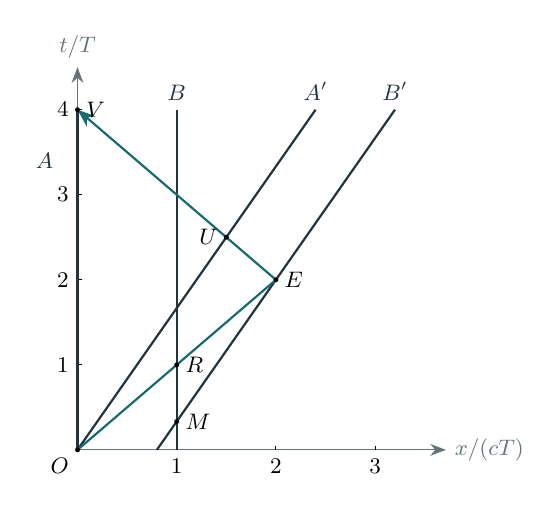
\begin{tikzpicture}[scale=0.9,transform shape]
\draw[axis] (0,0)--(5.2,0) node[right] {$x/(cT)$};\draw[axis] (0,0)--(0,5.4) node[above] {$t/T$};
\foreach \v in {1,2,3}
  \draw ({1.4*\v},.06)--({1.4*\v},0) node[below] {$\v$};
\foreach \v in {1,2,3,4}
  \draw (.065,{1.2*\v})--(0,{1.2*\v}) node[left] {$\v$};
\draw[object] (0,0)--(0,4.8) node[pos=.85,left=6pt] {$A$};\draw[object] (1.4,0)--(1.4,4.8) node[above] {$B$};
\draw[object] (0,0)--(3.36,4.8) node[above] {$A'$};\draw[object] (1.12,0)--(4.48,4.8) node[above] {$B'$};
\draw[motion] (0,0)--(2.8,2.4)--(0,4.8);
\fill (0,0) circle(.035) node[below left] {$O$};\fill (1.4,.4) circle(.035) node[right] {$M$};
\fill (1.4,1.2) circle(.035) node[right] {$R$};\fill (2.8,2.4) circle(.035) node[right] {$E$};
\fill (2.1,3) circle(.035) node[left] {$U$};\fill (0,4.8) circle(.035) node[right] {$V$};\end{tikzpicture}
\figcaption{解图近试.4C\quad $\beta=0.6$的实际事件图：$R$为$B$收光，$E$为$B^\prime$收光回发，$U$为$A^\prime$收回光，$V$为$A$收回光}
\end{minipage}\end{center}


\Needspace{13\baselineskip}

\pdfbookmark[2]{第 5 题 磁场轨迹与两体反应的粒子鉴别}{q5}

\section*{第 5 题\quad 磁场轨迹与两体反应的粒子鉴别}\label{q:5}


低速$K^-$介子与静止质子$p$反应，产生一个$\pi^+$介子和一个未知粒子$x$，初始总动量近似为零。两产物在垂直纸面向内的匀强磁场中运动，轨迹如图；磁感应强度$B=1.70\,\mathrm T$，测得$\pi^+$轨迹半径$R_1=34.0\,\mathrm{cm}$。
\begin{enumerate}
\item 求未知粒子电荷和轨迹半径$R_2$。
\item 用下表确定$x$的静能与粒子名称，并说明两产物速度对应的非相对论近似是否适用。
\end{enumerate}
反应时间很短，忽略磁场在反应过程中的外冲量，忽略入射$K^-$的动能；产物运动中磁场不做功。可用$c=3.00\times10^8\,\mathrm{m/s}$、$e=1.60\times10^{-19}\,\mathrm C$。

\begin{longtable}{@{}l c r c@{}}
\toprule 粒子 & 符号 & 静能$m_0c^2/\mathrm{MeV}$ & 电荷$/e$\\\midrule
电子、正电子 & $e^-,e^+$ & $0.511$ & $-1,+1$\\
缪子 & $\mu^-,\mu^+$ & $105.7$ & $-1,+1$\\
带电$\pi$介子 & $\pi^-,\pi^+$ & $139.6$ & $-1,+1$\\
带电$K$介子 & $K^-,K^+$ & $493.8$ & $-1,+1$\\
质子 & $p$ & $938.3$ & $+1$\\
中子 & $n$ & $939.6$ & $0$\\
$\Lambda$粒子 & $\Lambda^0$ & $1115.4$ & $0$\\
正$\Sigma$粒子 & $\Sigma^+$ & $1189.4$ & $+1$\\
中性$\Sigma$粒子 & $\Sigma^0$ & $1192.3$ & $0$\\
负$\Sigma$粒子 & $\Sigma^-$ & $1197.2$ & $-1$\\
中性$\Xi$粒子 & $\Xi^0$ & $1314.3$ & $0$\\
负$\Xi$粒子 & $\Xi^-$ & $1320.8$ & $-1$\\
$\Omega$粒子 & $\Omega^-$ & $1675$ & $-1$\\
\bottomrule
\end{longtable}


\begin{center}\begin{minipage}{.98\linewidth}\centering
\begin{tikzpicture}[scale=.85,transform shape]

\foreach \x/\y in {-3/2,0/2,3/2,-3/-2,0/-2,3/-2}{\node at (\x,\y) {$\otimes$};}
\coordinate (P) at (0,.8);
\draw[motion] (P) arc[start angle=90,end angle=145,radius=3];
\draw[motion] (P) arc[start angle=90,end angle=35,radius=3];
\fill (P) circle (2pt) node[above] {$P$};
\draw[guide] (0,2.6)--(P) node[midway,right] {$K^-+p$};
\node[left] at (-2.46,-.48) {$\pi^+$};\node[right] at (2.46,-.48) {$x$};
\node at (0,-3) {$\boldsymbol B$垂直纸面向内};

\end{tikzpicture}
\figcaption{图近试.5\quad 两产物从反应点沿相反方向飞出，随后在磁场中向下弯曲。}
\end{minipage}\end{center}

\Needspace{6\baselineskip}\subsection*{解答}


图近试.5中两个产物从同一点沿相反切线方向飞出。反应前总电荷为$(-e)+e=0$，$\pi^+$带$+e$，所以
\[
\boxed{q_x=-e}.
\]
反应处总动量近似守恒，$\boldsymbol p_\pi+\boldsymbol p_x=0$，故两动量大小相等为$p$。磁场中$\mathrm dE/\mathrm dt=q(\boldsymbol v\times\boldsymbol B)\cdot\boldsymbol v=0$，所以每个产物的速率、洛伦兹因子和总能量各自保持恒定。由$\mathrm d\boldsymbol p/\mathrm dt=\mathrm d(\gamma m_0\boldsymbol v)/\mathrm dt=\gamma m_0\boldsymbol a$，再用圆周运动的$a=v^2/R$，磁场中的曲率由相对论动量决定：
\[
|q|vB=\frac{pv}{R},\qquad
\boxed{p=|q|BR}.
\]
静质量$m_0$保持不变，相对论动量为$\gamma m_0v$，曲率直接对应这个动量。两产物电荷绝对值相同，因此
\[
\boxed{R_2=R_1=34.0\,\mathrm{cm}}.
\]
\begin{center}\begin{minipage}{.98\linewidth}\centering
\begin{tikzpicture}[scale=.8,transform shape]

\foreach \x/\y in {-3/2,0/2,3/2,-3/-2,0/-2,3/-2}{\node at (\x,\y) {$\otimes$};}
\coordinate (P) at (0,.8);
\draw[motion] (P) arc[start angle=90,end angle=145,radius=3];
\draw[motion] (P) arc[start angle=90,end angle=35,radius=3];
\fill (P) circle (2pt) node[above] {$P$};
\draw[guide] (0,2.6)--(P) node[midway,right] {$K^-+p$};
\node[left] at (-2.46,-.48) {$\pi^+$};\node[right] at (2.46,-.48) {$x$};
\node at (0,-3) {$\boldsymbol B$垂直纸面向内};

\draw[force] (-.3,.8)--(-2,.8) node[midway,above] {$\boldsymbol p_\pi$};
\draw[force] (.3,.8)--(2,.8) node[midway,above] {$\boldsymbol p_x$};
\draw[motion] (-1,.6)--(-1,-.8) node[below] {$\boldsymbol F_\pi$};
\draw[motion] (1,.6)--(1,0.342324541) node[below] {$\boldsymbol F_x$};
\node at (-3.8,.8) {$+e$};\node at (3.8,.8) {$-e$};

\end{tikzpicture}
\figcaption{解图近试.5A\quad 动量反向、电荷反号，两个洛伦兹力同向；各自速度由动量和总能量决定。}
\end{minipage}\end{center}
解图近试.5A把相反的动量与两个向下洛伦兹力分别标出，力箭头长度各自正比于速率：正粒子初向左、负粒子初向右，磁场向内，二者轨迹都向下弯。若向右为$x$正向、向上为$y$正向，磁场为$-B\hat{\boldsymbol z}$，正粒子初速$-v_\pi\hat{\boldsymbol x}$给出磁力$-ev_\pi B\hat{\boldsymbol y}$；负粒子初速$+v_x\hat{\boldsymbol x}$也给出磁力$-ev_xB\hat{\boldsymbol y}$。两个力的方向相同，大小随各自速率而定，向心加速度也分别由各自圆周运动确定。曲率方向由此与电荷守恒相符。

曲率测量先给出动量大小。已知$\pi^+$的静质量后，它的速率与总能量便可由动量确定；未知粒子仍有静质量和速率两个待求量，仅用等动量关系还只有一个独立约束。系统的总能量守恒补上第二个关系，先确定$x$的总能量，再由同一动量分离出静能。这一顺序使每条守恒关系都对应一个明确的未知量。先由$\pi^+$曲率求动量，再用能量守恒鉴别$x$：
\[
p=eBR_1=(1.60\times10^{-19})(1.70)(0.340)
=9.25\times10^{-20}\,\mathrm{kg\,m/s}.
\]
乘$c$并以$1\,\mathrm{MeV}=1.60\times10^{-13}\,\mathrm J$换算，
\[
pc\simeq\frac{(9.25\times10^{-20})(3.00\times10^8)}
{1.60\times10^{-13}}\,\mathrm{MeV}
\simeq173\,\mathrm{MeV}.
\]
从未取整的乘积$p=9.248\times10^{-20}\,\mathrm{kg\,m/s}$计算，$pc=2.7744\times10^{-11}\,\mathrm J$，除以每MeV的焦耳值可保留为$173.4$MeV。令$X=pc$、$M_\pi=m_\pi c^2$，动量关系$p=\gamma_\pi m_\pi v_\pi$平方后给出$X^2=M_\pi^2\beta_\pi^2/(1-\beta_\pi^2)$，即$\beta_\pi=X/\sqrt{X^2+M_\pi^2}$。其总能量为$M_\pi/\sqrt{1-\beta_\pi^2}$。保留中间有效数字取$pc\simeq173.4\,\mathrm{MeV}$，则
\[
E_\pi=\sqrt{(pc)^2+(m_\pi c^2)^2}
=\sqrt{(173.4)^2+(139.6)^2}\,\mathrm{MeV}
\simeq222.6\,\mathrm{MeV}.
\]
\begin{center}\begin{minipage}{.98\linewidth}\centering
\begin{tikzpicture}[scale=.8,transform shape]

\draw[object] (0,0) rectangle (9,1.1);
\draw[object] (1.4,0)--(1.4,1.1);
\node at (.7,.55) {$E_\pi$};\node at (5.2,.55) {$E_x$};
\draw[axis,<->] (0,1.8)--(9,1.8) node[midway,above] {$W=m_Kc^2+m_pc^2$};
\draw[motion] (1.2,-1.4)--(-.4,-1.4) node[midway,below] {$p$};
\draw[motion] (7.8,-1.4)--(9.4,-1.4) node[midway,below] {$p$};
\node[align=center] at (1.2,-3.2) {$E_\pi^2=(pc)^2+(m_\pi c^2)^2$};
\node[align=center] at (7.8,-4.3) {$m_xc^2=\sqrt{E_x^2-(pc)^2}$};
\node at (4.5,3) {先由曲率求共同动量，再分配总能量};

\end{tikzpicture}
\figcaption{解图近试.5B\quad 能量分段示意；总能量与静能通过共同动量联系。}
\end{minipage}\end{center}
解图近试.5B用能量分配图将初始静能分到两个产物。初始总能量为
\[
E_{\rm in}\simeq m_Kc^2+m_pc^2=493.8+938.3=1432.1\,\mathrm{MeV}.
\]
因此
\[
E_x=E_{\rm in}-E_\pi\simeq1209.5\,\mathrm{MeV}.
\]
由动量与总能量的关系$v/c=pc/E$，两产物速度为
\[
\frac{v_\pi}{c}=\frac{173.4}{222.6}\simeq0.779,\qquad
\frac{v_x}{c}=\frac{173.4}{1209.5}\simeq0.143.
\]
由上式，$F_\pi/F_x=v_\pi/v_x=E_x/E_\pi\simeq5.43$，对应解图A两个向下力箭头的长度比。两者具有相同动量，速度关系也可写成$v_x=(E_\pi/E_x)v_\pi$，所以$v_\pi$约为$2.34\times10^8$米每秒，$v_x$约为$4.30\times10^7$米每秒。这个$E_x$由静能与动能相加组成，查表前从共同动量中分离出静能。由$E_x=\gamma_xm_xc^2$，静能为$E_x\sqrt{1-v_x^2/c^2}$；将$v_x/c=pc/E_x$代入即得到下面的不变质量式。由不变质量关系，
\[
\boxed{m_xc^2=\sqrt{E_x^2-(pc)^2}
\simeq1197\,\mathrm{MeV}}.
\]
它带$-e$，静能接近表中$1197.2\,\mathrm{MeV}$的$\Sigma^-$，故
\[
\boxed{x=\Sigma^-}.
\]
若使用更精确的$c$，同一曲率给$pc\simeq173.28\,\mathrm{MeV}$，静能约$1197.1\,\mathrm{MeV}$，鉴别结论相同。

用同一测得的 $pc=173.4\,\mathrm{MeV}$ 来比较动能近似。解图近试.5C 上，$\pi^+$ 和 $x$ 的相对论动能分别约为 $83.0$ 和 $12.5\,\mathrm{MeV}$。若取非相对论动能 $p^2/(2m_0)=(pc)^2/(2m_0c^2)$，代入各自静能后得
\[
T_{\pi,{\rm nr}}\simeq107.7\,\mathrm{MeV},\qquad
T_{x,{\rm nr}}\simeq12.6\,\mathrm{MeV}.
\]
用未舍入值比较，非相对论式分别高估约 $30\%$ 和 $0.5\%$。因此 $\pi^+$ 的动能要用相对论式，$x$ 的动能可用非相对论式作粗估；精确鉴别静能时，两产物都用同一个能量—动量关系。磁场不做功，曲线上的动能在粒子沿圆弧运动时各自保持。
图近试.5的静能表用于最后的电荷与质量共同辨认。先由守恒确定负电荷，再把1197MeV附近的静能与负电荷候选比较，电子、缪子、$\pi^-$、$K^-$均太轻，$\Xi^-$和$\Omega^-$则更重，$\Sigma^-$与所测曲率和总能量相符。精度由$B$、半径和所用常数的有效位数控制，中间计算保留位数可避免把总能量舍入误差放大到静能反演中。解图近试.5C画两产物在共同动量下的动能曲线；各自产物总能量由动能加静能得到，轻产物分得较多的动能。
\begin{center}\begin{minipage}{.98\linewidth}\centering
\begin{tikzpicture}[scale=0.72,transform shape]
\draw[axis] (0,0)--(6.2,0);\draw[axis] (0,0)--(0,3.4000000000000004);
\draw[thin,color=muted] (0.0000000,0)--(0.0000000,-.07);\node[below] at (0.0000000,-.09) {$0$};
\draw[thin,color=muted] (3.0000000,0)--(3.0000000,-.07);\node[below] at (3.0000000,-.09) {$100$};
\draw[thin,color=muted] (5.2020000,0)--(5.2020000,-.07);\node[below] at (5.2020000,-.09) {$173.4$};
\draw[thin,color=muted] (6.0000000,0)--(6.0000000,-.07);\node[below] at (6.0000000,-.09) {$200$};
\draw[thin,color=muted] (0,0.0000000)--(-.07,0.0000000);\node[left] at (-.09,0.0000000) {$0$};
\draw[thin,color=muted] (0,1.4545455)--(-.07,1.4545455);\node[left] at (-.09,1.4545455) {$50$};
\draw[thin,color=muted] (0,2.9090909)--(-.07,2.9090909);\node[left] at (-.09,2.9090909) {$100$};
\node[anchor=west] at (6.32,0) {共同动量乘$c$（MeV）};\node[above right] at (0,3.45) {动能（MeV）};
\draw[guide] (5.202,0)--(5.202,2.4145);
\draw[traj] plot coordinates {(0.0000000,0.0000000) (0.0250000,0.0000724) (0.0500000,0.0002894) (0.0750000,0.0006512) (0.1000000,0.0011575) (0.1250000,0.0018085) (0.1500000,0.0026040) (0.1750000,0.0035439) (0.2000000,0.0046282) (0.2250000,0.0058567) (0.2500000,0.0072292) (0.2750000,0.0087458) (0.3000000,0.0104060) (0.3250000,0.0122099) (0.3500000,0.0141573) (0.3750000,0.0162478) (0.4000000,0.0184813) (0.4250000,0.0208576) (0.4500000,0.0233763) (0.4750000,0.0260373) (0.5000000,0.0288403) (0.5250000,0.0317850) (0.5500000,0.0348710) (0.5750000,0.0380980) (0.6000000,0.0414658) (0.6250000,0.0449740) (0.6500000,0.0486221) (0.6750000,0.0524099) (0.7000000,0.0563370) (0.7250000,0.0604029) (0.7500000,0.0646072) (0.7750000,0.0689496) (0.8000000,0.0734295) (0.8250000,0.0780466) (0.8500000,0.0828004) (0.8750000,0.0876903) (0.9000000,0.0927161) (0.9250000,0.0978770) (0.9500000,0.1031727) (0.9750000,0.1086026) (1.0000000,0.1141662) (1.0250000,0.1198629) (1.0500000,0.1256923) (1.0750000,0.1316537) (1.1000000,0.1377467) (1.1250000,0.1439706) (1.1500000,0.1503248) (1.1750000,0.1568088) (1.2000000,0.1634220) (1.2250000,0.1701637) (1.2500000,0.1770333) (1.2750000,0.1840303) (1.3000000,0.1911540) (1.3250000,0.1984038) (1.3500000,0.2057789) (1.3750000,0.2132789) (1.4000000,0.2209029) (1.4250000,0.2286504) (1.4500000,0.2365207) (1.4750000,0.2445131) (1.5000000,0.2526270) (1.5250000,0.2608615) (1.5500000,0.2692162) (1.5750000,0.2776902) (1.6000000,0.2862829) (1.6250000,0.2949935) (1.6500000,0.3038214) (1.6750000,0.3127658) (1.7000000,0.3218261) (1.7250000,0.3310015) (1.7500000,0.3402913) (1.7750000,0.3496948) (1.8000000,0.3592112) (1.8250000,0.3688399) (1.8500000,0.3785800) (1.8750000,0.3884309) (1.9000000,0.3983918) (1.9250000,0.4084621) (1.9500000,0.4186408) (1.9750000,0.4289274) (2.0000000,0.4393211) (2.0250000,0.4498211) (2.0500000,0.4604267) (2.0750000,0.4711371) (2.1000000,0.4819517) (2.1250000,0.4928696) (2.1500000,0.5038902) (2.1750000,0.5150127) (2.2000000,0.5262363) (2.2250000,0.5375603) (2.2500000,0.5489839) (2.2750000,0.5605065) (2.3000000,0.5721273) (2.3250000,0.5838455) (2.3500000,0.5956605) (2.3750000,0.6075714) (2.4000000,0.6195776) (2.4250000,0.6316783) (2.4500000,0.6438728) (2.4750000,0.6561603) (2.5000000,0.6685402) (2.5250000,0.6810117) (2.5500000,0.6935741) (2.5750000,0.7062267) (2.6000000,0.7189687) (2.6250000,0.7317995) (2.6500000,0.7447183) (2.6750000,0.7577244) (2.7000000,0.7708171) (2.7250000,0.7839958) (2.7500000,0.7972597) (2.7750000,0.8106081) (2.8000000,0.8240403) (2.8250000,0.8375557) (2.8500000,0.8511535) (2.8750000,0.8648331) (2.9000000,0.8785938) (2.9250000,0.8924349) (2.9500000,0.9063558) (2.9750000,0.9203557) (3.0000000,0.9344340) (3.0250000,0.9485901) (3.0500000,0.9628233) (3.0750000,0.9771329) (3.1000000,0.9915183) (3.1250000,1.0059788) (3.1500000,1.0205139) (3.1750000,1.0351228) (3.2000000,1.0498049) (3.2250000,1.0645597) (3.2500000,1.0793864) (3.2750000,1.0942845) (3.3000000,1.1092533) (3.3250000,1.1242923) (3.3500000,1.1394007) (3.3750000,1.1545781) (3.4000000,1.1698238) (3.4250000,1.1851372) (3.4500000,1.2005177) (3.4750000,1.2159648) (3.5000000,1.2314778) (3.5250000,1.2470563) (3.5500000,1.2626995) (3.5750000,1.2784069) (3.6000000,1.2941781) (3.6250000,1.3100123) (3.6500000,1.3259091) (3.6750000,1.3418679) (3.7000000,1.3578881) (3.7250000,1.3739693) (3.7500000,1.3901108) (3.7750000,1.4063121) (3.8000000,1.4225728) (3.8250000,1.4388922) (3.8500000,1.4552700) (3.8750000,1.4717054) (3.9000000,1.4881981) (3.9250000,1.5047475) (3.9500000,1.5213531) (3.9750000,1.5380144) (4.0000000,1.5547309) (4.0250000,1.5715022) (4.0500000,1.5883277) (4.0750000,1.6052069) (4.1000000,1.6221395) (4.1250000,1.6391248) (4.1500000,1.6561625) (4.1750000,1.6732520) (4.2000000,1.6903930) (4.2250000,1.7075849) (4.2500000,1.7248272) (4.2750000,1.7421196) (4.3000000,1.7594617) (4.3250000,1.7768528) (4.3500000,1.7942927) (4.3750000,1.8117809) (4.4000000,1.8293169) (4.4250000,1.8469003) (4.4500000,1.8645307) (4.4750000,1.8822078) (4.5000000,1.8999310) (4.5250000,1.9176999) (4.5500000,1.9355142) (4.5750000,1.9533735) (4.6000000,1.9712773) (4.6250000,1.9892252) (4.6500000,2.0072169) (4.6750000,2.0252520) (4.7000000,2.0433301) (4.7250000,2.0614508) (4.7500000,2.0796137) (4.7750000,2.0978185) (4.8000000,2.1160648) (4.8250000,2.1343522) (4.8500000,2.1526804) (4.8750000,2.1710489) (4.9000000,2.1894575) (4.9250000,2.2079058) (4.9500000,2.2263934) (4.9750000,2.2449201) (5.0000000,2.2634853) (5.0250000,2.2820889) (5.0500000,2.3007305) (5.0750000,2.3194097) (5.1000000,2.3381262) (5.1250000,2.3568797) (5.1500000,2.3756699) (5.1750000,2.3944964) (5.2000000,2.4133590) (5.2250000,2.4322573) (5.2500000,2.4511909) (5.2750000,2.4701597) (5.3000000,2.4891632) (5.3250000,2.5082013) (5.3500000,2.5272735) (5.3750000,2.5463796) (5.4000000,2.5655193) (5.4250000,2.5846924) (5.4500000,2.6038984) (5.4750000,2.6231372) (5.5000000,2.6424085) (5.5250000,2.6617119) (5.5500000,2.6810472) (5.5750000,2.7004141) (5.6000000,2.7198125) (5.6250000,2.7392418) (5.6500000,2.7587020) (5.6750000,2.7781928) (5.7000000,2.7977139) (5.7250000,2.8172650) (5.7500000,2.8368459) (5.7750000,2.8564563) (5.8000000,2.8760960) (5.8250000,2.8957647) (5.8500000,2.9154623) (5.8750000,2.9351883) (5.9000000,2.9549427) (5.9250000,2.9747251) (5.9500000,2.9945354) (5.9750000,3.0143733) (6.0000000,3.0342385)};
\draw[traj] (.1,-1.05)--(.7,-1.05);\node[right] at (.85,-1.05) {$\pi$ 的动能};\draw[dashed,thick,color=warm] plot coordinates {(0.0000000,0.0000000) (0.0250000,0.0000084) (0.0500000,0.0000338) (0.0750000,0.0000759) (0.1000000,0.0001350) (0.1250000,0.0002110) (0.1500000,0.0003038) (0.1750000,0.0004135) (0.2000000,0.0005401) (0.2250000,0.0006835) (0.2500000,0.0008439) (0.2750000,0.0010211) (0.3000000,0.0012151) (0.3250000,0.0014261) (0.3500000,0.0016539) (0.3750000,0.0018986) (0.4000000,0.0021602) (0.4250000,0.0024387) (0.4500000,0.0027340) (0.4750000,0.0030462) (0.5000000,0.0033753) (0.5250000,0.0037212) (0.5500000,0.0040841) (0.5750000,0.0044638) (0.6000000,0.0048603) (0.6250000,0.0052738) (0.6500000,0.0057041) (0.6750000,0.0061512) (0.7000000,0.0066153) (0.7250000,0.0070962) (0.7500000,0.0075940) (0.7750000,0.0081086) (0.8000000,0.0086401) (0.8250000,0.0091885) (0.8500000,0.0097537) (0.8750000,0.0103358) (0.9000000,0.0109348) (0.9250000,0.0115506) (0.9500000,0.0121833) (0.9750000,0.0128328) (1.0000000,0.0134992) (1.0250000,0.0141825) (1.0500000,0.0148826) (1.0750000,0.0155996) (1.1000000,0.0163334) (1.1250000,0.0170841) (1.1500000,0.0178516) (1.1750000,0.0186360) (1.2000000,0.0194372) (1.2250000,0.0202553) (1.2500000,0.0210902) (1.2750000,0.0219420) (1.3000000,0.0228106) (1.3250000,0.0236961) (1.3500000,0.0245984) (1.3750000,0.0255175) (1.4000000,0.0264535) (1.4250000,0.0274064) (1.4500000,0.0283760) (1.4750000,0.0293625) (1.5000000,0.0303659) (1.5250000,0.0313860) (1.5500000,0.0324231) (1.5750000,0.0334769) (1.6000000,0.0345475) (1.6250000,0.0356350) (1.6500000,0.0367394) (1.6750000,0.0378605) (1.7000000,0.0389985) (1.7250000,0.0401532) (1.7500000,0.0413248) (1.7750000,0.0425133) (1.8000000,0.0437185) (1.8250000,0.0449405) (1.8500000,0.0461794) (1.8750000,0.0474351) (1.9000000,0.0487075) (1.9250000,0.0499968) (1.9500000,0.0513029) (1.9750000,0.0526258) (2.0000000,0.0539655) (2.0250000,0.0553220) (2.0500000,0.0566953) (2.0750000,0.0580854) (2.1000000,0.0594923) (2.1250000,0.0609159) (2.1500000,0.0623564) (2.1750000,0.0638136) (2.2000000,0.0652877) (2.2250000,0.0667785) (2.2500000,0.0682861) (2.2750000,0.0698104) (2.3000000,0.0713516) (2.3250000,0.0729095) (2.3500000,0.0744842) (2.3750000,0.0760757) (2.4000000,0.0776839) (2.4250000,0.0793089) (2.4500000,0.0809506) (2.4750000,0.0826092) (2.5000000,0.0842844) (2.5250000,0.0859765) (2.5500000,0.0876853) (2.5750000,0.0894108) (2.6000000,0.0911531) (2.6250000,0.0929121) (2.6500000,0.0946879) (2.6750000,0.0964804) (2.7000000,0.0982896) (2.7250000,0.1001156) (2.7500000,0.1019583) (2.7750000,0.1038178) (2.8000000,0.1056939) (2.8250000,0.1075868) (2.8500000,0.1094965) (2.8750000,0.1114228) (2.9000000,0.1133659) (2.9250000,0.1153256) (2.9500000,0.1173021) (2.9750000,0.1192953) (3.0000000,0.1213052) (3.0250000,0.1233318) (3.0500000,0.1253751) (3.0750000,0.1274351) (3.1000000,0.1295117) (3.1250000,0.1316051) (3.1500000,0.1337152) (3.1750000,0.1358419) (3.2000000,0.1379854) (3.2250000,0.1401455) (3.2500000,0.1423222) (3.2750000,0.1445157) (3.3000000,0.1467258) (3.3250000,0.1489526) (3.3500000,0.1511960) (3.3750000,0.1534562) (3.4000000,0.1557329) (3.4250000,0.1580263) (3.4500000,0.1603364) (3.4750000,0.1626631) (3.5000000,0.1650065) (3.5250000,0.1673665) (3.5500000,0.1697431) (3.5750000,0.1721364) (3.6000000,0.1745463) (3.6250000,0.1769728) (3.6500000,0.1794159) (3.6750000,0.1818757) (3.7000000,0.1843521) (3.7250000,0.1868451) (3.7500000,0.1893546) (3.7750000,0.1918809) (3.8000000,0.1944237) (3.8250000,0.1969831) (3.8500000,0.1995591) (3.8750000,0.2021516) (3.9000000,0.2047608) (3.9250000,0.2073866) (3.9500000,0.2100289) (3.9750000,0.2126878) (4.0000000,0.2153633) (4.0250000,0.2180554) (4.0500000,0.2207640) (4.0750000,0.2234891) (4.1000000,0.2262309) (4.1250000,0.2289892) (4.1500000,0.2317640) (4.1750000,0.2345554) (4.2000000,0.2373633) (4.2250000,0.2401877) (4.2500000,0.2430287) (4.2750000,0.2458862) (4.3000000,0.2487603) (4.3250000,0.2516509) (4.3500000,0.2545579) (4.3750000,0.2574815) (4.4000000,0.2604216) (4.4250000,0.2633782) (4.4500000,0.2663513) (4.4750000,0.2693409) (4.5000000,0.2723470) (4.5250000,0.2753696) (4.5500000,0.2784087) (4.5750000,0.2814642) (4.6000000,0.2845362) (4.6250000,0.2876247) (4.6500000,0.2907297) (4.6750000,0.2938511) (4.7000000,0.2969889) (4.7250000,0.3001433) (4.7500000,0.3033140) (4.7750000,0.3065013) (4.8000000,0.3097049) (4.8250000,0.3129250) (4.8500000,0.3161615) (4.8750000,0.3194145) (4.9000000,0.3226838) (4.9250000,0.3259696) (4.9500000,0.3292718) (4.9750000,0.3325904) (5.0000000,0.3359254) (5.0250000,0.3392768) (5.0500000,0.3426446) (5.0750000,0.3460288) (5.1000000,0.3494294) (5.1250000,0.3528463) (5.1500000,0.3562796) (5.1750000,0.3597293) (5.2000000,0.3631954) (5.2250000,0.3666778) (5.2500000,0.3701766) (5.2750000,0.3736917) (5.3000000,0.3772232) (5.3250000,0.3807710) (5.3500000,0.3843351) (5.3750000,0.3879156) (5.4000000,0.3915124) (5.4250000,0.3951255) (5.4500000,0.3987550) (5.4750000,0.4024007) (5.5000000,0.4060628) (5.5250000,0.4097411) (5.5500000,0.4134358) (5.5750000,0.4171467) (5.6000000,0.4208739) (5.6250000,0.4246174) (5.6500000,0.4283772) (5.6750000,0.4321533) (5.7000000,0.4359456) (5.7250000,0.4397542) (5.7500000,0.4435790) (5.7750000,0.4474201) (5.8000000,0.4512774) (5.8250000,0.4551509) (5.8500000,0.4590407) (5.8750000,0.4629467) (5.9000000,0.4668690) (5.9250000,0.4708074) (5.9500000,0.4747621) (5.9750000,0.4787329) (6.0000000,0.4827200)};
\draw[dashed,thick,color=warm] (.1,-1.48)--(.7,-1.48);\node[right] at (.85,-1.48) {$x$ 的动能};
\fill[accent] (5.202,2.4145) circle(.045) node[above left=2pt] {$T_\pi$};
\fill[warm] (5.202,.3635) circle(.045) node[above left=2pt] {$T_x$};\end{tikzpicture}
\figcaption{解图近试.5C\quad 虚线标出题给曲率对应的共同动量，交点给出两产物的动能 $T_\pi$ 与 $T_x$。}
\end{minipage}\end{center}


\end{document}
